\documentclass[11pt,twoside,a4paper,fleqn]{book} 
%\documentclass[11pt,twoside,a4paper,fleqn,draft]{book} 


%--- Packages to use
%
\usepackage[]{fancyhdr}   
\usepackage[]{natbib}
\usepackage{alltt}
\usepackage{times}
\usepackage{lscape}         % landscape mode of a single page
\usepackage[]{longtable}    % allow tables longer than one page
\usepackage{makeidx}        % index of terms
\usepackage{tabularx}       % allows line breaking in table columns
\usepackage{algorithm}      % for describing algorithms with pseudo-code
\usepackage{algorithmic}
\usepackage{ifthen}
\usepackage{ifpdf}
\usepackage{xr-hyper}
\usepackage{fancyvrb}
\usepackage{xcolor}


%--- Margins
%
\voffset-1.5cm
\headheight16pt
\headsep1.1cm
\textheight23cm
\hoffset-1.3cm
\oddsidemargin2.2cm
\textwidth14.0cm


%--- Headings
%
\pagestyle{fancy}
\renewcommand{\chaptermark}[1]{\markboth{#1}{}}
\renewcommand{\sectionmark}[1]{\markright{\thesection\ #1}}
\fancyhf{}
\fancyhead[LE,RO]{\small{\sc\thepage}}
\fancyhead[LO]{\small{\scshape\rightmark}}
\fancyhead[RE]{\small{\scshape\leftmark}}
\renewcommand{\headrulewidth}{0.5pt}
\renewcommand{\footrulewidth}{0pt}
\fancypagestyle{plain}{%
  \fancyhead{}
  \renewcommand{\headrulewidth}{0pt}
}  


%--- Some layout commands
%
\sloppy
\raggedbottom
\hbadness=10000
\makeindex
\bibliographystyle{agu}


%--- Some fixes

%- To avoid hyperref error:
\newcommand{\theHalgorithm}{\theHchapter.\arabic{algorithm}}

%- Width of the caption in longtable:
\setlength{\LTcapwidth}{0.9\textwidth} 

%- Change brace type for comments in algorithmic
\renewcommand{\algorithmiccomment}[1]{(#1)}


%--- Symbol definitions
%

% This file defines the general math macros.
% Mathematical symbols used only once, or for a particular purpose, 
% should not be included here. Note that the scalar quantities exist 
% in a subscript version, and it is not necessary to define macros for
% all possible subscripts of a variable.
% A lot of macros have been defined for the Rodgers formalism is it
% used extensively.

% If you add new definitions, please try to follow the rules below to
% get a naming scheme as consistent as possible. Just check how a 
% similar macro is defined and use it as an example.

% Patrick Eriksson 2001-03-13

%-----------------------------------------------------------------------------

% Most of the macros are named by putting 3-letters acronyms together. 
% The acronyms are mainly formed by taking the first letter and the two 
% first following consonants. The list below shows the used acronyms.
% Please, if you introduce a new acronym, add it to this list.
%
% altitude     Alt
% angel        Ang
% average      Avr
% azimuthal    Azm
% constant     Cns
% contribution Cnt
% covariance   Cvr
% derivative   Drv
% error        Err
% frequency    Frq
% forward      Frw
% function     Fnc
% identity     Idn
% inverse      Inv
% kernel       Krn
% latitude     Lat       (exception from general naming scheme)
% length       Lng
% longitude    Lon       (exception from general naming scheme)
% matrix       Mtr
% measurement  Msr
% model        Mdl
% partial      Prt
% population   Ppl
% pressure     Prs
% radius       Rds
% retrieval/ed Rtr
% sensor       Sns
% size         Sze
% space        Spc
% state        Stt
% style        Stl
% symbol       Smb
% temperature  Tmp
% transfer     Trf
% transmission Trn
% transpose    Trp
% wavelength   Wvl
% vector       Vct
% zenith       Znt
%
% a priori                              Apr
% monochromatic pencil beam intensity   Mpi
% optical thickness                     Oth
% weighting function                    Wfn

% For other terms or features, use as far as possible complete strings to get 
% macros with clear names.


%--- General math ------------------------------------------------------------

% Vector style
\newcommand{\VctStl}[1]     {\ensuremath{\mathbf{#1}}}

% Matrix style
\newcommand{\MtrStl}[1]     {\ensuremath{\mathbf{#1}}}

% The identity matrix
\newcommand{\IdnMtr}        {\MtrStl{1}}  

% Scalar or matrix inverse
\newcommand{\Inv}           {^{-1}}  

% Vector or matrix transpose
\newcommand{\Trp}           {^T}  

% Size symbol
\newcommand{\SzeSmb}        {\ensuremath{\in}}  

% Vector space
\newcommand{\VctSpc}[1]     {\ensuremath{\mathbf{R}^#1}}

% Matrix space
\newcommand{\MtrSpc}[2]     {\ensuremath{\mathbf{R}^{#1 \times #2}}}

% Vector length (simple)
\newcommand{\VctLng}        {\ensuremath{n}}  
\newcommand{\aVctLng}[1]    {\ensuremath{n_{#1}}}  

% Index (to vector, matrix ...)
\newcommand{\Ind}           {\ensuremath{i}}  
\newcommand{\aInd}[1]       {\ensuremath{i_{#1}}}  

% Differential d
\newcommand{\DiffD}         {\ensuremath{\mathrm{d}}}  

% Partial d
\newcommand{\PartD}         {\ensuremath{\partial}}  

% Real and Imaginary part
\renewcommand{\Re}            {\ensuremath{\mathrm{Re}}}
\renewcommand{\Im}            {\ensuremath{\mathrm{Im}}}

% Ensemble average
\newcommand{\EnsAvr}[1]        {\ensuremath{\left\langle #1 \right\rangle}}

% Absolute Value
\newcommand{\Abs}[1]          {\ensuremath{\left| #1 \right| }}   

% *10^#1
\newcommand{\topowerten}[1]   {\ensuremath{\cdot10^{#1}}}

% degrees
\newcommand{\degree}          {\ensuremath{^\circ}}

% 1/2
\newcommand{\half} {\ensuremath{\textstyle\frac{1}{2}}}


%--- Physical constants ------------------------------------------------------

% Speed of light in vaccum [m/s]
\newcommand{\speedoflight}   {\ensuremath{c}}  

% Planck constant [Js]
\newcommand{\planckCns}      {\ensuremath{h}}  

% Boltzmann constant [J/K]
\newcommand{\boltzmannCns}   {\ensuremath{k_b}}  

% Avogadro's number [molec/kg]
\newcommand{\avogadrosCns}   {\ensuremath{N_a}}  


%--- The Rodgers formalism ---------------------------------------------------

% True (natural) forward model
\newcommand{\trueFrwMdl}       {\ensuremath{F}}  

% Discrete forward model
\newcommand{\FrwMdl}           {\ensuremath{\mathcal{F}}}  

% Inverse model  
\newcommand{\InvMdl}           {\ensuremath{\mathcal{I}}}  

% Transfer model  
\newcommand{\TrfMdl}           {\ensuremath{\mathcal{T}}}  

% A priori symbol
\newcommand{\AprSmb}           {\ensuremath{_a}}  

% Measurement vector
\newcommand{\MsrVct}           {\VctStl{y}}  

% Vector of monochromatic pencil beam intensities
\newcommand{\MpiVct}           {\VctStl{i}}  

% Vector of monochromatic pencil beam intensities with subscript
\newcommand{\aMpiVct}[1]       {\MpiVct\ensuremath{_{#1}}}

% Measurement error vector
\newcommand{\MsrErrVct}        {\ensuremath{\varepsilon}}  

% State vector 
\newcommand{\SttVct}           {\VctStl{x}}  
\newcommand{\aSttVct}[1]       {\SttVct\ensuremath{_{#1}}}
\newcommand{\aSttVctTrp}[1]    {\SttVct\ensuremath{_{#1}\Trp}}
\newcommand{\SttElm}           {\ensuremath{x}}  
\newcommand{\aSttElm}[1]       {\SttElm\ensuremath{_{#1}}}

% A priori state vector 
\newcommand{\AprSttVct}        {\SttVct\AprSmb}

% Retrieved state vector
\newcommand{\RtrVct}           {\ensuremath{\hat{\SttVct}}}

% Forward model parameter vector
\newcommand{\FrwMdlVct}        {\VctStl{b}}  

% A priori forward model parameter vector 
\newcommand{\AprFrwMdlVct}     {\FrwMdlVct\AprSmb}

% A forward model parameters vector with subscript
\newcommand{\aFrwMdlVct}[1]    {\FrwMdlVct\ensuremath{_{#1}}}
\newcommand{\aFrwMdlVctTrp}[1] {\FrwMdlVct\ensuremath{_{#1}\Trp}}

% Inverse model parameters
\newcommand{\InvMdlVct}        {\VctStl{c}}  

% Weighting function matrix
\newcommand{\WfnMtr}           {\MtrStl{K}}
\newcommand{\aWfnMtr}[1]       {\WfnMtr\ensuremath{_{#1}}}
\newcommand{\aWfnMtrTrp}[1]    {\WfnMtr\ensuremath{_{#1}\Trp}}

% Contribution function matrix
\newcommand{\CtrFncMtr}        {\MtrStl{D_y}}  

% Averaging kernel matrix
\newcommand{\AvrKrnMtr}        {\MtrStl{A}}  
\newcommand{\aAvrKrnMtr}[1]    {\AvrKrnMtr\ensuremath{_{#1}}}

% Sensor (and data reduction) matrix
\newcommand{\SnsMtr}           {\MtrStl{H}} 
\newcommand{\aSnsMtr}[1]       {\SnsMtr\ensuremath{_{#1}}} 

% Transformation between vector spaces
\newcommand{\VctTrfMtr}        {\MtrStl{B}}  

% Covariance matrix
\newcommand{\CvrMtr}           {\MtrStl{S}}


% --- Special functions ------------------------------------------------------

% The Planck function
\newcommand{\Planck}     {\ensuremath{B}}  


% --- General scalar quantities ----------------------------------------------
%
% All quantities shall have a subscript version named as aXxx.

% Altitude (above geoid)
\newcommand{\Alt}        {\ensuremath{z}}  
\newcommand{\aAlt}[1]    {\ensuremath{z_{#1}}}

% Azimuthal angle
\newcommand{\AzmAng}     {\ensuremath{\omega}}  
\newcommand{\aAzmAng}[1] {\ensuremath{\omega_{#1}}}  

% Frequency
\newcommand{\Frq}        {\ensuremath{\nu}}  
\newcommand{\aFrq}[1]    {\ensuremath{\nu_{#1}}}  

% Wavelength
\newcommand{\Wvl}        {\ensuremath{\lambda}}  
\newcommand{\aWvl}[1]    {\ensuremath{\lambda_{#1}}}  

% Latitude
\newcommand{\Lat}        {\ensuremath{\alpha}}  
\newcommand{\aLat}[1]    {\ensuremath{\alpha_{#1}}}  

% Length along the propagation path
\newcommand{\PpathLng}        {\ensuremath{l}}  
\newcommand{\aPpathLng}[1]    {\ensuremath{l_{#1}}}  

% Longitude
\newcommand{\Lon}        {\ensuremath{\beta}}  
\newcommand{\aLon}[1]    {\ensuremath{\beta_{#1}}}  

% Monochromatic pencil beam intensity
\newcommand{\Mpi}        {\ensuremath{I}}  
\newcommand{\aMpi}[1]    {\ensuremath{I_{#1}}}  

% Optical depth
\newcommand{\Oth}        {\ensuremath{\tau}}  
\newcommand{\aOth}[1]    {\ensuremath{\tau_{#1}}}  

% Transmission
\newcommand{\Trn}        {\ensuremath{t}}  
\newcommand{\aTrn}[1]    {\ensuremath{t_{#1}}}  
\newcommand{\TrnMat}     {\MtrStl{T}}
\newcommand{\aTrnMat}[1] {\ensuremath{\MtrStl{T}_{#1}}}  

% Pressure
\newcommand{\Prs}        {\ensuremath{P}}  
\newcommand{\aPrs}[1]    {\ensuremath{P_{#1}}}  

% Pressure altitude
\newcommand{\PrsAlt}     {\ensuremath{\zeta}}  
\newcommand{\aPrsAlt}[1] {\ensuremath{\zeta_{#1}}}  

% Radius
\newcommand{\Rds}        {\ensuremath{r}}  
\newcommand{\aRds}[1]    {\ensuremath{r_{#1}}}  

% Refractive index
\newcommand{\Rfr}        {\ensuremath{n}}  
\newcommand{\aRfr}[1]    {\ensuremath{n_{#1}}}  
\newcommand{\RealRfr}    {\ensuremath{n'}}  
\newcommand{\ImagRfr}    {\ensuremath{n''}}  

% Speed
\newcommand{\Spd}        {\ensuremath{v}}  
\newcommand{\aSpd}[1]    {\ensuremath{v_{#1}}}

% Temperature
\newcommand{\Tmp}        {\ensuremath{T}}  
\newcommand{\aTmp}[1]    {\ensuremath{T_{#1}}}  

% Zenith angle
\newcommand{\ZntAng}     {\ensuremath{\psi}}  
\newcommand{\aZntAng}[1] {\ensuremath{\psi_{#1}}}  

% Winds
\newcommand{\Wind}        {\ensuremath{v}}  
\newcommand{\WindWE}      {\ensuremath{v_u}}  
\newcommand{\WindSN}      {\ensuremath{v_v}}  
\newcommand{\WindVe}      {\ensuremath{v_w}}  


% --- Radiative transfer quantities -------------------

% Stokes vector
\newcommand{\StoVec}    {\ensuremath{{\bf s}}}
\newcommand{\aStoVec}[1]{\ensuremath{{\bf s}_{#1}}}
\newcommand{\StoI}      {\ensuremath{I}}
\newcommand{\aStoI}[1]  {\ensuremath{I_{#1}}}
\newcommand{\StoQ}      {\ensuremath{Q}}
\newcommand{\aStoQ}[1]  {\ensuremath{Q_{#1}}}
\newcommand{\StoU}      {\ensuremath{U}}
\newcommand{\StoV}      {\ensuremath{V}}

% Degree of polarisation
\newcommand{\DgrPlr}      {\ensuremath{p}}

% Propagation direction and position
\newcommand{\PDir}      {\ensuremath{{\bf \hat{n}}}}
\newcommand{\PPos}      {\ensuremath{{\bf r}}}

% Total extinction matrix
\newcommand{\ExtMat}    {\ensuremath{{\bf K}}}
\newcommand{\aExtMat}[1]{\ensuremath{{\bf K}_{#1}}}

% Absorption matrix
\newcommand{\AbsMat}    {\ensuremath{{\bf A}}}
\newcommand{\aAbsMat}[1]{\ensuremath{{\bf A}_{#1}}}

% Total absorption vector
\newcommand{\AbsVec}    {\ensuremath{{\bf a}}}
\newcommand{\aAbsVec}[1]{\ensuremath{{\bf a}_{#1}}}     

% Emission source vector
\newcommand{\EmsVec}    {\ensuremath{{\bf b}}}

% Source vector
\newcommand{\SrcVec}    {\ensuremath{{\bf j}}}
\newcommand{\aSrcVec}[1]{\ensuremath{{\bf j}_{#1}}}     

% Phase matrix
\newcommand{\PhaMat}    {\ensuremath{{\bf Z}}}
\newcommand{\aPhaMat}[1]{\ensuremath{{\bf Z}_{#1}}}

% Scattering matrix
\newcommand{\ScaMat}    {\ensuremath{{\bf F}}}
\newcommand{\aScaMat}[1]{\ensuremath{{\bf F}_{#1}}}

% Particle density
\newcommand{\PDen}      {\ensuremath{n^p}}

% Radiation field
\newcommand{\IFld}      {\ensuremath{{\mathcal I}}}
% Radiation field index
\newcommand{\aIFld}[1]  {\ensuremath{{\mathcal I}^{(#1)}}}

% Scattered field
\newcommand{\SFld}      {\ensuremath{{\mathcal S}}}

% Scattered field index
\newcommand{\aSFld}[1]  {\ensuremath{{\mathcal S}^{(#1)}}}

% Scattering Integral vector
\newcommand{\SVec}      {\ensuremath{{\bf s}}}

% Amplitude matrix
\newcommand{\AmpMat}    {\ensuremath{{\bf S}}}

% Phase matrix
\newcommand{\TraMat}    {\ensuremath{{\bf T}}}
\newcommand{\aTraMat}[1]{\ensuremath{{\bf T}_{#1}}}

% Amplitude matrix index
\newcommand{\IAmp}      {\ensuremath{i_{amp}}}

% Single extinction matrix
\newcommand{\SExMat}    {\ensuremath{{\bf L}}}
\newcommand{\aSExMat}[1]{\ensuremath{{\bf L}^{#1}}}     

% Scattered field
\newcommand{\ScaInt}    {\ensuremath{{\bf S}}}

% Identity matrix
\newcommand{\IdnMat}    {\ensuremath{{\bf E}}}

% Scattering zenith angle
\newcommand{\ScaZa}     {\ensuremath{{\psi_s}}}

% Scattering azimuth angle
\newcommand{\ScaAa}     {\ensuremath{{\omega_s}}}

% Particle type index
\newcommand{\IPart}     {\ensuremath{{i_{part}}}}

%Inverse Wave Impendance
\newcommand{\InvImp} %
      {\ensuremath{\sqrt{\textstyle{\frac{\epsilon}{\mu}}}}}    

% Micrometer
\newcommand{\mum}          {\ensuremath{\mu m}}

% Incoming direction
\newcommand{\inc}       {\mathrm{inc}}

% Scattered direction
\newcommand{\sca}       {\mathrm{sca}}

% Mass content
\newcommand{\mc}       {\ensuremath{MC}}

% Ice mass content
\newcommand{\imc}       {\ensuremath{IMC}}

% effective radius
\newcommand{\Reff}       {\ensuremath{R_{eff}}}


% --- Quantities concerning scalar gas absorption  -------------------

% Absorption coefficient
\newcommand{\AbsCoef}    {\ensuremath{{\alpha}}}
\newcommand{\aAbsCoef}[1]{\ensuremath{{\alpha}_{#1}}}

% Total absorption coefficient
\newcommand{\AbsCoefTot} {\aAbsCoef{\mbox{\footnotesize total}}}

% Absorption cross section
\newcommand{\AbsXsec}    {\ensuremath{{\kappa}}}
\newcommand{\aAbsXsec}[1]{\ensuremath{{\kappa}_{#1}}}

% Number density:
\newcommand{\Den}    {\ensuremath{{n}}}
\newcommand{\aDen}[1]{\ensuremath{{n}_{#1}}}


% --- Intensity for different polarisation components  -------------------

\newcommand{\Iv}      {\ensuremath{I_v}}
\newcommand{\Ih}      {\ensuremath{I_h}}
\newcommand{\Ipff}    {\ensuremath{I_{+45^\circ}}}
\newcommand{\Imff}    {\ensuremath{I_{-45^\circ}}}
\newcommand{\Irhc}    {\ensuremath{I_{rhc}}}
\newcommand{\Ilhc}    {\ensuremath{I_{lhc}}}


% --- Brightness temperature  -------------------

\newcommand{\BT}      {\aTmp{B}}


%--- Plotting line styles ----------------------------------------------------

\def \lsolid     {\mbox{------}}
\def \ldashed    {\mbox{--~--~--}}
\def \ldashdot   {\mbox{--~$\cdot$~--}}
\def \ldotted    {\mbox{$\cdot~\cdot~\cdot$}}


% --- Misc  -------------------
\newcommand{\chem}[1] {{\ensuremath{\mathrm{#1}}}}





%--- PDF/LaTeX specific options
\ifpdf
  \usepackage{graphicx}    % includegraphics
  \DeclareGraphicsExtensions{.pdf}
  \usepackage{color}
  \definecolor{DarkRed}{rgb}{0.5,0,0}
  \usepackage
    [pdftex,                         % or dvips
     colorlinks=true,
     linkcolor=DarkRed,
     citecolor=DarkRed,
     urlcolor=DarkRed,
%     pdftitle={ARTS User Guide},
%     pdfauthor={The ARTS development team},
%     pdfsubject={},
%     pdfkeywords={},
%     bookmarks=true,
%     bookmarksopen=false,
%     pdfpagemode=None,
%     plainpages=false,
%     pdfpagelabels
      ]
  {hyperref}
  \setcounter{tocdepth}{3}
\else
  \usepackage{graphicx}    % includegraphics
  \DeclareGraphicsExtensions{.eps}
  \setcounter{tocdepth}{1}
\fi


%--- Command definitions -----------------------------------------------------

%- Document history
\newcommand{\starthistory} {\begin{table}[b]  \begin{tabular}{l p{11cm}} 
                             \hline {\bf History} & \\ }
\newcommand{\stophistory}  {\end{tabular} \end{table} }


%- Symbol table
\newcommand{\startsymbols} {\begin{table} \begin{center} 
                            \caption{Examples of symbols used in this chapter,
                            the corresponding notation in the ARTS source code
                            and a short description of the quantity. }
                            \begin{tabular}{l l l}
                            {\bf Here} & {\bf In ARTS} & {\bf Description} 
                            \\ \hline \\ } 
\newcommand{\stopsymbols}  {\\ \hline \end{tabular} 
                           \end{center} \end{table}}      
\newcommand{\startsymbolswithunits} 
                   {\begin{table} \begin{center} 
                            \caption{Examples of symbols used in this chapter,
                            the corresponding notation in the ARTS source code
                            and a short description of the quantity. }
                   \begin{tabular}{l l l l}
                   {\bf Here} & {\bf Unit} & {\bf In ARTS} & {\bf Description} 
                   \\ \hline \\ } 
\newcommand{\stopsymbolswithunits} {\stopsymbols}

% ARTS Web address
\newcommand{\artsserver}{http://www.radiativetransfer.org/}

% Docserver for this ARTS version
\newcommand{\docserver}{docserver-trunk/}

%- Command to link to a URL on the ARTS web server
% takes the subpath (without leading / !!!) as input
\newcommand{\artsurl}[1]{\href{http://www.radiativetransfer.org/#1}{http://www.radiativetransfer.org/#1}}

%- Command to create link to ARTS built-in documentation. (Consider
% using \wsmindex, \wsvindex, etc., instead. They use this command
% implicitly.  But direct use may be useful if you use the same term
% several times in a short section, and don't want all of these
% occurrences to be in the index.)
% Underscores must be escaped by leading backslash!
\newcommand{\builtindoc}[1]{\href{\artsserver\docserver all/#1}{#1}}

%- Command to write an internal ARTS variable, internal function, or
% file name with special style. Anything that does not have built-in
% documentation. Also for other things that are code,
% but inside the text. Use the "code" environment for longer pieces of
% code.
% Underscores must be escaped by leading backslash!
\newcommand{\shortcode}[1]{\texttt{#1}}

%- Define verbatim environment for arts code examples.
% (For longer pieces of code, for in-text use "\shortcode".)
% This is the only code command where you do not have to escape
% underscores. 
\DefineVerbatimEnvironment{code}{Verbatim}{fontsize=\small}


%- Commands for easy indexing of terms
%
% Underscores must be escaped by leading backslash!
%
% Index command to use when text and index reference are equal. Otherwise
% the normal \index command must be used.
\newcommand{\textindex}[1]{#1\index{#1}} 
%
% Index command to make index for a workspace method. It writes out the
% function name in verbatim style and makes an index reference.
\newcommand{\wsmindex}[1]{\builtindoc{#1}\index{workspace methods!#1}} 
%
% Index command to make index for workspace variable. Works as \wsmindex.
\newcommand{\wsvindex}[1]{\builtindoc{#1}\index{workspace variables!#1}}
%
% Index command to make index for workspace agenda. Works as \wsmindex.
\newcommand{\wsaindex}[1]{\builtindoc{#1}\index{workspace agendas!#1}} 
%
% Index command to make index for a ARTS file. Works as \wsmindex.
\newcommand{\fileindex}[1]{\shortcode{#1}\index{ARTS files!#1}}
%
% Index command to make index for an internal function. Works as \wsmindex.
\newcommand{\funcindex}[1]{\shortcode{#1}\index{internal ARTS functions!#1}}
%
% Index command to make index for a ARTS data structure. Works as \wsmindex.
\newcommand{\typeindex}[1]{\shortcode{#1}\index{data types!#1}}


%- For FIXMEs:
\newcommand{\FIXME}[1]{\textcolor{gray}{\bfseries FIXME: #1}}


%- Names of the different documentation documents:
\newcommand{\user}{\emph{ARTS User Guide}}
\newcommand{\developer}{\emph{ARTS Developer Guide}}
\newcommand{\theory}{\emph{ARTS Theory}}

%------------------------------------------------------------------------------



%%% Local Variables: 
%%% mode: latex
%%% TeX-master: t
%%% End: 


% External documents for cross references:
\externaldocument[U-]{arts_user}
\externaldocument[T-]{arts_theory}

%===   Start of report   ===================================================
\begin{document}


%--- Title page
%
% To suppress hyperref warning about duplicate page labels:
\renewcommand{\thepage}{title \arabic{page}} 

\thispagestyle{plain}
\begin{center}
  \vspace*{1cm}
  {\Huge \bf ARTS Developer Guide\\}
  \vspace*{1cm}
  {\large edited by \\}
  \vspace*{1cm}
  {\Large \bf Stefan Buehler and Patrick Eriksson}\\
   \vspace*{2cm}
   {\large \today\\
    ARTS Version \input{auto_version}
   }
\end{center}
\vspace*{\fill}
{\normalsize \bf
  \noindent
  The content and usage of ARTS are not only described by this
  document. An overview of ARTS documentation and help features is
  given in \user, Section \ref{U-sec:concept:doc}. For continuous reports on
  changes of the source code and this user guide, subscribe to the
  ARTS developers mailing list at \artsurl{contact/}.

  We welcome gladly comments and reports on errors in the document.
  Send then an e-mail to: \verb|patrick.eriksson (at) chalmers.se| or 
  \verb|sbuehler (at) uni-hamburg.de|.

  If you use data generated by ARTS in a scientific
  publication, then please mention this and cite the most
  appropriate of the ARTS publications that are summarized on
  \artsurl{/docs/}.
}

\newpage                          
\thispagestyle{empty}
\vspace*{\fill}
\noindent
\begin{code}
Copyright (C) 2000-2015
Stefan Buehler <sbuehler (at) uni-hamburg.de>
Patrick Eriksson <patrick.eriksson (at) chalmers.se>

The ARTS program is free software; you can redistribute it
and/or modify it under the terms of the GNU General Public
License as published by the Free Software Foundation; either
version 2, or (at your option) any later version.

This program is distributed in the hope that it will be
useful, but WITHOUT ANY WARRANTY; without even the implied
warranty of MERCHANTABILITY or FITNESS FOR A PARTICULAR
PURPOSE. See the GNU General Public License for more
details. 

You should have received a copy of the GNU General Public
License along with the program; if not, write to the Free
Software Foundation, Inc., 59 Temple Place - Suite 330,
Boston, MA 02111-1307, USA. 
\end{code}



%--- Contributing authors -----------------------------------------------------
%
\newpage
\thispagestyle{plain}
%
\begin{center}
  {\Large \bf Contributing authors}
\end{center}
\vspace*{10mm}
\begin{tabular}{lp{10mm}l}
  \hline
  {\bf Author/email} & & {\bf Main contribution(s)} \\
  \hline
  Stefan Buehler$^a$ & & Editor, Sections \ref{sec:development}, \ref{sec:workspace},
  \ref{sec:matpack} and \ref{sec:interpolation}.\\
  sbuehler (at) uni-hamburg.de & &        \\
 \hline
  Mattias Ekstr\"om$^b$ & & Section \ref{sec:matpack:sparse}. \\
  \hline
  Claudia Emde$^c$ & & Section \ref{sec:lin_alg}.\\
  claudia.emde (at) dlr.de & & \\
  \hline
  Patrick Eriksson$^b$ &  & Editor. \\
  patrick.eriksson (at) chalmers.se & & \\
  \hline
  Oliver Lemke$^a$ & & Section \ref{sec:griddedfields}.\\
  olemke (at) core-dump.info & & \\
 \hline
  Sreerekha T.R.$^c$ & & Section \ref{sec:integration}.\\
  \hline
  &&\\
\end{tabular}

\noindent
The present address is given for active contributors, while for others
the address to the institute where the work was performed is given:\\
$^a$ Meteorological Institute, University of Hamburg, Bundesstr. 55,
20146 Hamburg, Germany.\\
$^b$ Department of Space, Earth and Environment, Chalmers University of Technology,
SE-41296 Gothenburg, Sweden. \\
$^c$ Institute of Environmental Physics, University of Bremen, P.O. Box 33044, 
28334 Bremen, Germany. \\
%$^d$ Department of Computer Science, Electrical and Space Engineering,
%Division of Space Technology, Lule{\aa} University of Technology, Box
%812, 98128 Kiruna, Sweden. \\


%--- Create an empty page
%
\newpage
\thispagestyle{empty}
\rule{0pt}{10pt}
\newpage

\pagenumbering{roman}
\tableofcontents

\cleardoublepage
\pagenumbering{arabic}
     

% ===========================================================================
% === The chapters
%============================================================================


%
% To start the document, use
%  \chapter{...}
% For lover level, sections use
%  \section{...}
%  \subsection{...}
%
\chapter{The art of developing ARTS}
 \label{sec:development}

%
% Document history, format:
%  \starthistory
%    date1 & text .... \\
%    date2 & text .... \\
%    ....
%  \stophistory
%
\starthistory
  020425 & Stefan Buehler: Put this part back in the AUG. Updated.\\
  000728 & Stefan Buehler: Added stuff about build system and howto cut a release. \\
  000615 & Created by Stefan Buehler.\\
\stophistory

%
% Symbol table, format:
%  \startsymbols
%    ... & \shortcode{...} & text ... \\
%    ... & \shortcode{...} & text ... \\
%    ....
%  \stopsymbols
%
%

%
% Introduction
%
The aim of this section is to describe how the program is organized and to give
detailed instructions how to make extensions. That means, it is addressed to the
ARTS developers, not the users. If you only want to use ARTS, you should not
need to read it. \textbf{But if you want to make changes or additions, you
  should definitely read this carefully, since it can save you a lot of work to
  understand how things are organized.}

\section{Organization}
%====================
\label{sec:development:org}
 
ARTS is written in C++ and uses the cross-platform, open-source build system
CMake (\url{http://www.cmake.org/}). It is organized in a similar manner as most
GNU packages. The top-level ARTS directory is either called \shortcode{arts} or
\shortcode{arts-x.y}, where x.y is the release number. It contains various
sub-directories, notably \shortcode{doc} for documentation, \shortcode{src} for
the C++ source code, The document that you are reading right now, the ARTS
Developer Guide, is located in \shortcode{doc/uguide}.

There are two different versions of the ARTS package: The development version
and the end-user version. Both contain the complete source code, the only
difference is that the developers version is where active development takes
place.

The end-user version contains everything that you need in order to compile and
install ARTS in a fairly automatic manner. The only thing you should need is an
ANSI-C++ compiler, and the CMake utility. Please see files
\fileindex{arts/README} and \fileindex{arts/INSTALL} for installation
instructions. We are aiming to support recent version of the GNU and clang C++
compilers.

\section{The ARTS build system}
%============================

As mentioned above, CMake is used to build the ARTS package. A good introduction
to the CMake system can be found in:
\begin{quote}
  \url{http://www.cmake.org/cmake/project/about.html}
\end{quote}


\subsection{Configure options}
%========================================

For development, it is recommended to build ARTS using the
\shortcode{RelWithDebInfo} configuration (see below), which aims to provide a
reasonable trade-off between debugging capability and performance. To use ARTS
in production, however, it is important to perform a release build, which is
therefore set as the default configuration.

\begin{description}
\item[\shortcode{-DCMAKE\_BUILD\_TYPE=RelWithDebInfo}:] This is the build option
  that should be used for development, as it will make it easier to track down
  errors in the code. It does, however, not disable all compiler optimization,
  so as to still provide reasonable performance.
\item[\shortcode{-DCMAKE\_BUILD\_TYPE=Release}:] Removes '-g' from
the compiler flags and includes \shortcode{\#define NDEBUG 1} in
\fileindex{config.h}. The central switch to turn off all debugging
features (index range checking for vectors, the trace facility,
assertions,...).
\item[\shortcode{-DCMAKE\_BUILD\_TYPE=Debug}:] This switch turns off all
  optimizations. This should only be used if the \shortcode{RelWithDebInfo}
  configuration makes debugging a given problem difficult.
\item[\shortcode{-DNO\_OPENMP=1}:] 
Disables the generation of multi-threaded code. CMake tries to detect if the compiler supports OpenMP and enables it by default.

\end{description}


\section{Coding conventions}
%===================
\label{sec:development:conv}

With the aim of improving quality and consistency of the code, all new code that
is added to ARTS should adhere to naming and formatting conventions from
Google's C++ programming guidelines
(\url{https://google.github.io/styleguide/cppguide.html#Formatting}). Adhering
to a well-defined coding style will make it much easier for your fellow ARTS
developers to understand and work with your code. A brief summary of the most
important programming style and formatting conventions is given below.


\subsection{Naming conventions}

Naming things is one of the two hard problems in computer science. Certainly,
there is no single best way to do it and even with the best names code can still
be bad. Yet still, the consistently naming of objects in your code will make it
much easier for other developers to read and understand your code.

In general, the use descriptive names in all your code is recommended.
Try to avoid abbreviations except when they are very common. Giving proper
names to objects increases the readability of the code and decreases the need
for explanatory comments.

\subsubsection{Variables}
Variable names should use lower-case letters. Words should be separated using
underscores:
  \begin{code}
  Index element_index = 0;
  Numeric t_surface = 0.0; // common abbreviation
  \end{code}

\subsubsection{Classes, structs and type names}
Classes, structs and user-defined type names should start with a capital letter
and use camel case to separate different words.
  \begin{code}
  class CovarianceMatrix {};
  \end{code}

\subsubsection{Class member variables}

Variables that are defined as data members of classes should be suffixed with
a underscore (\shortcode{\_}). This convention has the important advantage
that it allows inferring the scope of variables used inside definitions of
member functions.

  \begin{code}
  class CovarianceMatrix {
   private:
    Numeric *elements_;
  };
  \end{code}

\subsubsection{Constant names}
Names of constants should be prefixed with a lower-case k. Following words
should use camel case starting with a capital letter.
  \begin{code}
  const Numeric kAlmostPi = 3.0;
  \end{code}

\subsubsection{Function names}
Function names should start with a capital letter and words should
be separated using camel case.

  \begin{code}
  void InterpolateTo(const Vector &x_new) {
    ...
  }
  \end{code}

\subsection{Formatting}

The formatting, i.e. the layout of your code, should adhere strictly to the
Google guidelines. Google's indentation style is also supported by the
clang-format tool, which provides functionality for automatic formatting. A
format file for clang-format is provided in ARTS' top-level directory. Most
development environments provide support for clang-format, which makes following
these guidelines extremely easy.

\begin{itemize}
  \item Line length of 80 characters
  \item No tabs, only spaces
  \item 2 spaces per indentation level
  \item Opening brace \texttt{\{} of function/class/struct definition and if/for blocks on the same line
  \item No spaces on the inner side of the parentheses of the conditional
    expressions of if statements.
\end{itemize}

\subsection{ARTS-specific rules}

\subsubsection{Numeric types}

Never use \shortcode{float} or \shortcode{double} explicitly, use the type
\typeindex{Numeric} instead. This is set by CMake (to \shortcode{double} by
default). In the same way, use \typeindex{Index} for all integers. It can take
on positive or negative values and defaults to \shortcode{long}. To change the
default types, run \shortcode{cmake} with the options \shortcode{-DINDEX=long}
or \shortcode{-DNUMERIC=double}:

\begin{code}
cmake -DINDEX=int --DNUMERIC=float ..
\end{code}

Note that changing the numeric type to a lower precision type than
double might have unforseen impacts on the numerical precision and could
lead to wrong results. In a similar way, reducing the index type can
make it impossible to handle larger Vectors, Matrices or Tensors. The
maximum range of the index type determines the maximum number of
elements the container types can handle.

\subsection{Container types} Use \builtindoc{Vector} and
\builtindoc{Matrix} for mathematical vectors and matrices (with elements
of type \builtindoc{Numeric}). Use \shortcode{Array<something>} to
create an array of \shortcode{something}s.
Commonly used Arrays have been predefined, they have names like
\builtindoc{ArrayOfString}, \builtindoc{ArrayOfMatrix}, and so forth.

\subsection{Terminology}
Calculations are carried out in the so called workspace (WS), on
workspace variables (WSVs). A WSV is for example the variable
containing the absorption coefficients. The WSVs are manipulated by 
workspace methods (WSMs). The WSMs to use are specified in the
controlfile in the same order in which they will be
executed. 

\subsection{Global variables}
   Are not visible by default. To use them you have to declare them
   like this:
   \begin{quote}
   \shortcode{extern const Numeric PI;}
   \end{quote}
   which will make the global constant PI=3.14... available. Other important globals are:

   \begin{quote}
   \begin{tabular}{ll}
   \shortcode{full\_name}&         Full name of the program, including version.\\
   \shortcode{parameters}&        All command line parameters.\\
   \shortcode{basename}&          Used to construct output file names.\\
   \shortcode{out\_path}&          Output path.\\
   \shortcode{messages}&          Controls the verbosity level.\\
   \shortcode{wsv\_data}&          WSV lookup data.\\
   \shortcode{wsv\_group\_names}&   Lookup table for the names of \emph{types} of WSVs.\\
   \shortcode{WsvMap}&            The map associated with \shortcode{wsv\_data}. \\
   \shortcode{md\_data}&           WSM lookup data.\\
   \shortcode{MdMap}&             The map associated with \shortcode{md\_data}. \\
   \shortcode{workspace}&         The workspace itself.\\
   \shortcode{species\_data}&      Lookup information for spectroscopic species.\\
   \shortcode{SpeciesMap}&        The map associated with \shortcode{species\_data}.
   \end{tabular}
   \end{quote}
   The only exception from this rule are the output streams \shortcode{out0} to
   \shortcode{out3}, which are visible by default.

\subsection{Files}
Always use the \shortcode{open\_output\_file} and \shortcode{open\_input\_file}
functions to open files. This switches on exceptions, so that any
error occurring later on with this file will result in an
exception. (Currently not really implemented in the GNU compiler,
but please use it anyway.)

\subsection{Version numbers} 
The package version number is set in the \fileindex{VERSION} file in the top
level ARTS directory. It will be incremented by the ARTS maintainers when new
features or bug fixes have been added to ARTS, not on every commit. Never
change this number when working in your own branch. The major and/or minor
version number will be incremented on public releases. The micro version
indicates the addition of new features during development or bugfixes for
stable releases.

\subsection{Header files} 
The global header file \fileindex{arts.h} \emph{must} be included by every
file. Apart from that you have to see yourself what header files you
need. If you use functions from the C or C++ standard library, you
have to also include the appropriate header file.

\subsection{Documentation}
Doxygen is used to generate automatic source code documentation. See
\begin{quote}
  \url{http://www.stack.nl/\~dimitri/doxygen/}
\end{quote}
for information. There is a complete User manual there. At the moment
we only generate the output as HTML, although latex, man-page, and rtf
format is also possible. The HTML version is particularly useful for
source code browsing, since it includes the complete source code! You
should add Doxygen headers to the following:

\begin{enumerate}
\item Files
\item Classes (Including all private and public members)
\item Functions
\item Global Variables
\end{enumerate}

The documentation headers are comment blocks that look like the
examples below.

Doxygen supports several different comment block styles. Over the years,
probably all of them were used somewhere in ARTS. New code should follow the
Doxygen JavaDoc style. If you edit existing documentation, it is recommended
to convert it to the current style.

\subsubsection{File comment}

Each header and source code file should contain a doxygen comment stating the
original author, creation date and a short summary of its contents.

\begin{code}
/**
 * @file   dummy.cc
 * @author John Doe <john.doe (at) example.com>
 * @date   2011-03-02
 *
 * @brief  A dummy file.
 *
 * This file has no purpose at all,
 * it just servers as an example...
 */
\end{code}

\subsubsection{Function comment}

Each function should be preceeded with a doxygen comment.
It starts with a brief description, ending with a dot. Then follows a more
detailed description of the function's purpose and parameters.

The doxygen comment block should be put above the \emph{declaration} of the
function, i.e., in the \shortcode{.h} file.  If a function is only declared in
a \shortcode{.cc} file, the comment should be put there instead.

If arguments are modified by the function you should add
`[out]' after the \shortcode{@param} command, just like for the
parameter \shortcode{a} in the example below. If a parameter is both input
and output, it should say `[in,out]'. Parameters that are not modified inside
the function, e.g. passed by value or const reference, should carry an `[in]'.
The documentation for each parameter should start with a capital letter and
end with a period, like in the example below.

Author and date tags are not inserted by default, since they would be
overkill if you have many small functions. However, you should include
them for important functions.

\begin{code}
/** A dummy function.
 *
 * This function has no purpose at all,
 * it just serves as an example...
 *
 * @param[out]     a This parameter is initialized by the function.
 * @param[in,out]  b This parameter is modified by the function.
 * @param[in]      c This parameter is not changed by the function.
 *
 * @return   Dummy value computed from a and b.
 */
int dummy(int& a, int& b, int c);
\end{code}

\subsubsection{Classes and structs}

Classes und structs must be preceeded by a doxygen comment describing their
intent and purpose. A short description should be provided for each member
variable. Member function are documented as described in the previous section.

\begin{code}
/** Brief description of Foobar.
 *
 * Long description of Foobar.
 */
class FooBar {
 private:
  /** Number of elements. */
  Index nelem;
}
\end{code}

\subsubsection{Doxymacs for Emacs}
There is an Emacs package (Doxymacs) that makes the insertion of
documentation headers particularly easy. You can find documentation of
this on the Doxymacs webpage: \url{http://doxymacs.sourceforge.net/}.
To use it for ARTS (provided you have it), put the following in your
Emacs initialization file:

\begin{code}
    (require 'doxymacs)

    (setq doxymacs-doxygen-style "JavaDoc")

    (defun my-doxymacs-font-lock-hook ()
    (if (or (eq major-mode 'c-mode) (eq major-mode 'c++-mode))
    (progn
    (doxymacs-font-lock)
    (doxymacs-mode))))

    (add-hook 'font-lock-mode-hook 'my-doxymacs-font-lock-hook)

    (setq doxymacs-doxygen-root "../doc/doxygen/html/")
    (setq doxymacs-doxygen-tags "../doc/doxygen/arts.tag")
\end{code}

The only really important lines are the first two, where the second
line is the one selecting the style of documentation. The next block
just turns on syntax highlighting for the Doxygen headers, which looks
nice. The last two lines are needed if you want to use the tag lookup
features (see Doxymacs documentation if you want to find out what this
is).  The package allows you to automatically insert headers. The
standard key-bindings are:
\begin{quote}
    \begin{tabularx}{.8\hsize}{@{}lX}
        \texttt{C-c d ?} & look up documentation for the symbol under the point.\\
        \texttt{C-c d r} & rescan your Doxygen tags file.\\
        \texttt{C-c d f} & insert a Doxygen comment for the next function.\\
        \texttt{C-c d i} & insert a Doxygen comment for the current file.\\
        \texttt{C-c d ;} & insert a Doxygen comment for a member variable on the current line (like M-;).\\
        \texttt{C-c d m} & insert a blank multi-line Doxygen comment.\\
        \texttt{C-c d s} & insert a blank single-line Doxygen comment.\\
        \texttt{C-c d @} & insert grouping comments around the current region.\\
    \end{tabularx}
\end{quote}

You can call macros to insert certain types of doxygen comment by name:

\begin{itemize}
\item \shortcode{doxymacs-insert-file-comment}
\item \shortcode{doxymacs-insert-function-comment}
\item \shortcode{doxymacs-insert-blank-multiline-comment}
\item \shortcode{doxymacs-insert-blank-singleline-comment}
\end{itemize}


\section{Extending ARTS}
%======================
\label{sec:development:extending}

\subsection{How to add a workspace variable}
%---------------------------------------

You should read Section \ref{sec:agendas:wsvs} to understand what workspace
variables are. Here is just the practical description how a new
variable can be added.

\begin{enumerate}
\item Create a record entry in file \fileindex{workspace.cc}. (Just add
  another one of the \shortcode{wsv\_data.push\_back} blocks.) Take the
  already existing entries as templates. The ARTS concept works best
  if WSVs are only of a rather limited number of different types, so
  that generic WSMs can be used extensively, for example for IO.
  
  The name must be \emph{exactly} like you use it in the source code,
  because this is used to generate interface functions.
  
  Make sure that the documentation string you give explains the
  variable and its purpose well. \textbf{In particular, state the
    dimensions (in the case of matrices) and the units!} This string
  is used for the online documentation. Please take some time to write
  it carefully. Use the template at the beginning of function
  \shortcode{define\_wsv\_data()} in file \shortcode{workspace.cc} as a
  guideline. 

\item That's it!
\end{enumerate}


\subsection{How to add a workspace variable group}
%--------------------------------------------

You should read Section \ref{sec:agendas:wsvs} to understand what workspace
variable groups are. Here is just the practical description how a new
group can be added.

\begin{enumerate}
\item Add a \shortcode{wsv\_group\_names.push\_back("your\_type")} function to
  the function \shortcode{define\_wsv\_group\_names()} in \fileindex{groups.cc}.
  The name must be \emph{exactly} like you use it in the source code,
  because this is used to generate interface functions.
\item XML reading/writing routines are mandatory for each workspace variable
  group. Two steps are necessary to add xml support for the new group:
  \begin{enumerate}
  \item Implement an \shortcode{xml\_read\_from\_stream}
    and \shortcode{xml\_write\_to\_stream} function. Depending
    on the type of the group the implementation goes into one
    of the three files \fileindex{xml\_io\_basic\_types.cc},
    \fileindex{xml\_io\_compound\_types.cc}, or
    \fileindex{xml\_io\_array\_types.cc}. Basic types are for example Index
    or Numeric. Compound types are structures and classes. And array types are
    arrays of basic or compound types. Also add the function declaration in the
    corresponding \shortcode{.h} file.
  \item Add an explicit instantiation for
    \shortcode{xml\_read\_from\_file<GROUP>} and
    \shortcode{xml\_write\_to\_file<GROUP>} to \fileindex{xml\_io\_instantiation.h}.
  \end{enumerate}
\item If your new group does not implement the output operator
  (\shortcode{operator<<}), you have to add an explicit implementation
  of the \builtindoc{Print} function in \fileindex{m\_general.h} and
  \fileindex{m\_general.cc}.
\item That's it! (But as stated above, use this feature wisely)
\end{enumerate}



\subsection{How to add a workspace method}
%-------------------------------------
\label{sec:development:extending:wsm}

You should read Section \ref{sec:agendas:wsms} to understand what workspace
methods are. Here is just the practical description how a new
method can be added.

\begin{enumerate}
\item Create an entry in the function \funcindex{define\_md\_data} in file
  \fileindex{methods.cc}.  (Make a copy of an existing entry (one of the
  \shortcode{md\_data.push\_back(...)} blocks) and edit it to fit your new
  method.) Don't forget the documentation string! Please refer to the
  example at the beginning of the file to see how to format it.
\item Run:
  \shortcode{make}.
\item Look in \fileindex{auto\_md.h}. There is a new function prototype
  \begin{quote}
    \shortcode{void <YourNewMethod>(...)}
  \end{quote}
\item Add your function to one of the \shortcode{.cc} files which contain method
  functions. Such files must have names starting with \shortcode{m\_}. (See
  separate HowTo if you want to create a new source file.) The header
  of your function must be compatible with the prototype in \shortcode{auto\_md.h}.
\item Check that everything looks nice by running 
  \begin{quote}
    \shortcode{arts -d YourNewMethod}
  \end{quote}
  If necessary, change the documentation string.

\item Thats it!
\end{enumerate}


\subsection{How to add a source code file}
%---------------------------------------
\begin{enumerate}
\item Create your file. Names of files containing workspace methods should
  start with \shortcode{m\_}.
\item You have to register your file in the file
  \fileindex{src/CMakeLists.txt}. This file states which source files
  are needed for arts. In the usual case, you just have to add your
  \shortcode{.cc} file to the list of source files of the artscore
  library. Header files are not added to this list.
\item Go to \shortcode{src} and run: \shortcode{git add <my\_file>} to
  make your file known to git.
\end{enumerate}


\subsection{How to add a test case}
%---------------------------------------
\begin{enumerate}
\item Tests are located in subdirectories in the \fileindex{controlfiles}
  folder. Instrument specific test cases are in the
  \fileindex{controlfiles/instruments} folder, all other cases are
  located in the \fileindex{controlfiles/artscomponents} folder. Create
  a new subdirectory in the appropriate folder. If your test is closely
  related to another test case you can skip this step and instead add it
  to one of the existing subdirectories.
\item Create your own test controlfile. The filename should start
  with \fileindex{Test} followed by the name
  of the subdirectory it is located in, e.g.
  \fileindex{controlfiles/artscomponents/doit/TestDOIT.arts}.

  If the subdirectory contains more than one test controlfile,
  append a short descriptive text to the end of the filename like
  \fileindex{controlfiles/artscomponents/ montecarlo/TestMonteCarloGaussian.arts}.
\item Copy all required input files into the subdirectory. Input data that is
  shared among several test cases should be placed in
  \fileindex{controlfiles/testdata}.
\item Add an entry for your test case in
  \fileindex{controlfiles/CMakeLists.txt}.
\end{enumerate}


\subsection{How to add a particle size distribution}
%---------------------------------------
In \shortcode{m\_psd.cc}, add a workspace method \shortcode{psdPsdName}, where
\shortcode{PsdName} stands for the name or name tag of the new particle size
distribution (PSD) parametrization. (see Section~\ref{sec:development:extending:wsm}
for details). If several \shortcode{psdPsdName} methods are based on the same 
algorithm, add the algorithm as an internal function to \shortcode{psd.cc}.


\section{Version control}
%======================
\label{sec:development:cvs}

ARTS uses git for version control. The central or \textit{upstream} repository
is hosted on github (\url{https://github.com/atmtools/arts}). Contributions to
ARTS are handled via pull requests on github. This is the de-facto standard
workflow for open source development, so the time required to get familiar with
it is certainly a worthy investment. Contributing a new feature or bug-fix to
ARTS thus involves the following steps:

\begin{enumerate}
\item Fork the upstream repository
\item Clone the ARTS fork from \textit{your github account} onto your local
  workstation
\item Implement your changes
\item Commit and push your changes to your ARTS fork
\item Issue a pull request to merge your ARTS fork with the central repository
\item One of the ARTS core developers will review your code and help with the
  final integration
\end{enumerate}


The required steps are described below in more detail. Note that all of these
steps are so common to modern software development, that it is very easy to find
tutorials and manuals online that described them in more detail.


\subsection{Forking the central repository}

The forking of the central repository is through the web interface of
\url{github.com}. This will create a copy of the central repository in
\textit{your account}. This repository is your personal version of the ARTS
repository. You can change all you want here without breaking ARTS for anyone
else.

\subsection{Clone your ARTS fork}

So far your fork of ARTS exists only in your github account somewhere in
the \textit{cloud}. To really work with the code, you need to obtain a copy
of the code on your local workstation. This is done by \textit{cloning} the
repository from your account:
\begin{code}
  git clone https://github.com/<your_username>/arts
\end{code}

where \shortcode{your\_username} is the name of your github account. The
important point to note here is that you did not clone the central ARTS
repository from \url{github.com/atmtools} but the one from your account. As
explained above, this is your personal version of the ARTS repository
and you can do anything you want with it.

\subsection{Update your fork}

One consequences of the forking of the central ARTS repository is that the
fork in your own github account will not automatically be updated when
changes are made to the upstream repository. Before checking in your changes
into your repository it is therefore important that you update your repository
with the most recent changes made to the upstream repository. For this two
steps are required:

\begin{enumerate}
\item Register the upstream repository as remote repository for your local clone of your ARTS fork:
  \begin{code}
    git remote --add upstream https://github.com/atmtools/arts
  \end{code}
\item Rebase your code onto the newest changes from the upstream repository:
  \begin{code}
    git fetch upstream master
    git rebase -i upstream/master
  \end{code}
\end{enumerate}

The first step here needs to be performed only the first time you are going
through this process. Afterwards only the second step is required. A detailed
description of the rebase step can be found at \url{https://www.atlassian.com/git/tutorials/rewriting-history/git-rebase}.

\subsection{Commit and push your changes}

After implementing your changes, commit and push them to your ARTS fork. The
changes are now publicly available from your github account. Note that at this
point you can already share your code with others or across different machines.
It has, however, not yet been integrated into the upstream repository. That
means your changes are not yet affecting regular users of the ARTS development
version.

\subsection{Issuing a pull request}

Once your changes have been pushed to the ARTS repository in your github
account, you can issue a pull request. This is done most easily through the
github web interface. This will notify the ARTS core developers that you want to
integrate your changes into the upstream repository. On issuing your pull
request, the ARTS test-suite will be run on your code. If all tests pass, an
ARTS core developer will review your code and finally merge it into the central
repository.

\section{Debugging (use of assert)}
%================================
\label{sec:development:assert}
 
The idea behind assert is simple. Suppose that at a certain point in
your code, you expect two variables to be equal.  If this expectation
is a precondition that must be satisfied in order for the subsequent
code to execute correctly, you must assert it with a statement like
this:
\begin{quote}
\shortcode{assert(var1 == var2);}
\end{quote}

In general assert takes as argument a boolean expression. If the
boolean expression is true, execution continues. Otherwise the
\shortcode{abort} system call is invoked and the program execution is
stopped. If a bug prevents the precondition from being true, then you
can trace the bug at the point where the precondition breaks down
instead of further down in execution or not at all.  The \shortcode{assert} call
is implemented as a C preprocessor macro, so it can be enabled or
disabled at will. 

In ARTS, you don't have to do this manually, as long as your source file
includes \shortcode{arts.h} either directly or indirectly. Instead, assertions
are turned on and off with the global NDEBUG preprocessor macro, which is
set or unset automatically by the \shortcode{cmake} build configuration.
Assertions are enabled in the default \shortcode{cmake} build configuration
(\shortcode{-DCMAKE\_BUILD\_TYPE=RelWithDebInfo}). They are turned off in the
release configuration (\shortcode{-DCMAKE\_BUILD\_TYPE=Release}).

If your program is stopped by an assertion failure, then the first
thing you should do is to find out where the error happens. To do
this, run the program under the GDB debugger. First invoke
the debugger:
\begin{quote}
\shortcode{gdb arts}
\end{quote}
You have to give the full path to the ARTS executable.  Then set a
breakpoint at the assertion failure:
\begin{quote}
  \shortcode{(gdb) break \_\_assert\_fail}
\end{quote}
(Note the two leading underscores!) Now run the program: 
\begin{quote}
  \shortcode{(gdb) run}
\end{quote}

Instead of just exiting, under the debugger the program will be paused
when the assertion fails, and you will get back the debugger prompt.
Now type:
\begin{quote}
  \shortcode{(gdb) where} 
\end{quote}  
to see where the assertion failure happened. You can use the
\shortcode{print} command to look at the contents of variables and you
can use the \shortcode{up} and \shortcode{down} commands to navigate
the stack.  For more information, see the GDB documentation or type
\shortcode{help} at the prompt of GDB.

For ARTS, the assertion failures mostly happen inside the Tensor /
Matrix / Vector package (usually because you triggered a range check
error, i.e., you tried to read or write beyond array bounds). In this
case the \shortcode{up} command of GDB is particularly useful. If you
give this a couple of times you will finally end up in the part of
your code that caused the error.

Recommendation: In Emacs there is a special GDB mode. With this you
can very conveniently step through your code.

%%% Local Variables: 
%%% mode: latex
%%% TeX-master: "uguide"
%%% End: 


\chapter{The workspace}
%-------------------------------
\label{sec:workspace}

\starthistory
  110622 & Updated by Oliver Lemke.\\
  020605 & Created by Stefan Buehler.\\
\stophistory

This chapter deals with the main components of ARTS: \emph{Workspace
  variables}\index{workspace variables} (\textindex{WSVs}) and
\emph{workspace methods}\index{workspace methods} (\textindex{WSMs}).
Furthermore, it explains the use of \textindex{agendas}, a special
group of WSVs.

%To make the text easier to read, we will often use \emph{variables}
%as a synonym for workspace variables, and \emph{methods} as a synonmy
%for workspace methods. So:

%\begin{quote}
%\begin{tabular}{lclcl}
%  workspace variable &=& WSV &=& variable,\\
%  workspace method   &=& WSM &=& method
%\end{tabular}
%\end{quote}

\section{Implementation files}
%----------------------------
\label{sec:agendas:files}

The most important files are:
\begin{itemize}
\item \fileindex{workspace.cc}:\\
  Definition and documentation of WSVs.
\item\fileindex{methods.cc}:\\
  Definition and documentation of WSMs. The
  implementations of WSMs reside in files named
  \shortcode{m\_something.cc}.
\item \fileindex{agendas.cc}:\\
  Definition and documentation of agendas.
\end{itemize}
It is very likely that you will have to edit these. Less likely, but
possibly, you also have to edit:
\begin{itemize}
\item \fileindex{groups.cc}:\\
  Definition of WSV groups.
\end{itemize}

\vspace{2ex}
When ARTS is built, a number of source code files are generated
automatically. They are listed here in the order in which they are
generated: 
\begin{itemize}
\item \fileindex{auto\_workspace.h}:\\
  Generated from \shortcode{groups.cc}.
\item \fileindex{auto\_md.h}, \fileindex{auto\_md.cc}:\\
  Generated from \shortcode{auto\_workspace.h},
  \shortcode{agendas.cc}, \shortcode{groups.cc}, and \shortcode{methods.cc}.
\end{itemize}
This is achieved by a set of simple C++ programs:
\begin{itemize}
\item \fileindex{make\_auto\_workspace\_h.cc}
\item \fileindex{make\_auto\_md\_h.cc}
\item \fileindex{make\_auto\_md\_cc.cc}
\end{itemize}
The meaning of the names should be self-explanatory. There is one program
for each file to be generated.  The generation of the
\shortcode{auto\_} files happens automatically when you do a
\shortcode{make}. Therefore, never edit any of these files.

Next, there are some files that contain the internal implementation
of WSVs and WSMs. These are:
\begin{itemize}
\item \fileindex{wsv\_aux.h}:\\
  Implementation of class
  \typeindex{WsvRecord}, which stores the lookup information for one
  WSV, plus auxiliary stuff for the workspace.
\item \fileindex{methods.h}, \fileindex{methods\_aux.cc}:\\
  Implementation of class \typeindex{MdRecord}, which stores the
  lookup information for one WSM.
\end{itemize}

Finally, there are some files that contain the internal implementation
of agendas. These are:
\begin{itemize}
\item \fileindex{agenda\_class.h}, \fileindex{agenda\_class.cc}:\\
  Implementation of class \typeindex{MRecord}, which stores runtime
  information for one WSM, and class \typeindex{Agenda}, which stores
  an agenda.
\item \fileindex{agenda\_record.h}, \fileindex{agenda\_record.cc}:\\
  Implementation of class \typeindex{AgRecord}, which is used to store
  agenda lookup information.
\end{itemize}
  

\vspace{2ex} As mentioned above, you will not have to modify any of
the implementation files, they are listed here just for reference.
Normally, you only have to modify \shortcode{workspace.cc},
\shortcode{methods.cc}, and \shortcode{agendas.cc}.

\section{Workspace Variables or WSVs}
%--------------------------
\label{sec:agendas:wsvs}

All important variables in ARTS are WSVs. This means that they can be
manipulated by a list of WSMs, which is specified in the ARTS
controlfile. There exists a predefined list of possible WSVs. This
list defines the \emph{workspace}. One can think of each WSV as a
`slot' in the workspace: The WSV can be either \emph{set}, or
\emph{unset}. Set means that the WSV has a well-defined content, unset
means that it has no well-defined content. At the start of an ARTS job
all WSVs are unset.

WSVs are defined in the file \fileindex{workspace.cc}. A typical
definition looks like this:

\begin{code}
wsv_data.push_back
  (WsvRecord
   ( NAME( "f_grid" ),
     DESCRIPTION
     (
      "The frequency grid for monochromatic pencil beam\n"
      "calculations.\n"
      "\n"
      "Usage:      Set by the user.\n"
      "\n"
      "Unit:       Hz"
      ),
     GROUP( "Vector" )));
\end{code}

\noindent
All WSV definitions have the same three elements:
\begin{enumerate}
\item The \emph{name}, exactly the
  same name has to be used in the code.
\item The \emph{description}, which is normally much longer than in
  the example here. It must fully describe the WSV, its purpose, and
  its normal usage. See file \shortcode{workspace.cc} for instructions
  how to write the documentation.
\item The \emph{group} to which the WSV belongs. You can think of a
  group as something similar to a C++ data type. The WSV in the
  example belongs to the group \builtindoc{Vector}. The allowed groups
  are defined in file \fileindex{groups.cc}.
\end{enumerate}

\noindent
See Section \ref{sec:development:extending} for explicit
instructions how to add a new WSV to ARTS.

\section{Workspace Methods or WSMs}
%---------------------------------
\label{sec:agendas:wsms}

WSMs manipulate WSVs to produce other WSVs. There are three kinds of
WSMs:
\begin{enumerate}
\item Specific WSMs.
\item Generic WSMs.
\item Agenda WSMs.
\end{enumerate}
As in the case of WSVs, there is a central place in ARTS where
information on the available WSMs is stored. This place is the file
\fileindex{methods.cc}. It contains a record for each WSM. Here is an
example:

\begin{code}
md_data_raw.push_back
  ( MdRecord
    ( NAME( "r_geoidSpherical" ),
      DESCRIPTION
      (
       "Sets the geoid to be a perfect sphere.\n"
       "\n"
       "The radius of the sphere is selected by the generic argument r.\n"
      ),
      AUTHORS( "Patrick Eriksson" ),
      OUT( "r_geoid" ),
      GOUT(),
      GOUT_TYPE(),
      GOUT_DESC(),
      IN( "atmosphere_dim", "lat_grid", "lon_grid" ),
      GIN( "r" ),
      GIN_TYPE(    "Numeric" ),
      GIN_DEFAULT( NODEF     ),
      GIN_DESC( "Radius of the geoid sphere."),
      ));
\end{code}

\noindent
All WSM definitions have the same elements:
\begin{enumerate}
\item The \emph{NAME}, exactly as in the code.
\item The \emph{DESCRIPTION}. This must fully describe the WSM, its
  purpose, and its normal usage. See file \shortcode{methods.cc} for
  instructions how to write the documentation.
\item The \emph{OUT}. This is a list of WSV names.
All these WSVs are set by this WSM.
\item The \emph{GOUT}. This is a list descriptive names for the generic
outputs.
\item The \emph{GOUT\_TYPE}. This is a list of WSV group names.
This defines the group to which the generic output arguments must belong
(see below).
\item The \emph{GOUT\_DESC}, a list of short descriptions for the generic outputs.
\item The \emph{IN}. This is a list of WSV names.
All these WSVs are required as input by this WSM. This means they must have
been set before.
\item The \emph{GIN}, a list of descriptive names for the generic inputs.
\item The \emph{GIN\_TYPE}. This is a list of WSV group names.
This defines the group to which the generic input arguments must belong.
\item The \emph{GIN\_DEFAULT}, a list of default values for the generic inputs.
\shortcode{NODEF} means that the generic input has no default and the user has
to set it in the control file.
\item The \emph{GIN\_DESC}, a list of short descriptions for the generic inputs.
\end{enumerate}

\subsection{Specific WSMs}
%---------------------

\begin{code}
md_data_raw.push_back     
  ( MdRecord
    ( NAME( "p_gridFromGasAbsLookup" ),
      DESCRIPTION
      (
       "Sets *p_grid* to the frequency grid of *abs_lookup*.\n"
      ),
      AUTHORS( "Patrick Eriksson" ),
      OUT( "p_grid" ),
      GOUT(),
      GOUT_TYPE(),
      GOUT_DESC(),
      IN( "abs_lookup" ),
      GIN(),
      GIN_TYPE(),
      GIN_DEFAULT(),
      GIN_DESC()
      ));
\end{code}

For this type of WSM the output and input is fixed. Fields
\shortcode{GIN} and \shortcode{GOUT} are empty. The example
above belongs in this category. It sets the WSV \builtindoc{p\_grid}, using
the WSV \builtindoc{abs\_lookup} as input.

To call this method in the controlfile, you just have to write
\builtindoc{p\_gridFromGasAbsLookup}.

\subsection{Generic WSMs}
%--------------------

This class of WSMs is more powerful, because it can be applied to any
WSV that belongs to the right group. A good example is:

\begin{code}
md_data_raw.push_back
  ( MdRecord
    ( NAME( "VectorSetConstant" ),
      DESCRIPTION
      (
       "Creates a vector and sets all elements to the specified value.\n"
       "\n"
       "The vector length is determined by *nelem*.\n"
       ),
      AUTHORS( "Patrick Eriksson" ),
      OUT(),
      GOUT(      "v"      ),
      GOUT_TYPE( "Vector" ),
      GOUT_DESC( "Variable to initialize." ),
      IN( "nelem" ),
      GIN(         "value"   ),
      GIN_TYPE(    "Numeric" ),
      GIN_DEFAULT( NODEF     ),
      GIN_DESC(    "Vector value." )
      ));
\end{code}

\noindent
As you probably have guessed, this WSM resizes the output vector to have \builtindoc{nelem} elements and sets all elements to the given \shortcode{value}.
You would use it as follows:

\begin{code}
IndexSet(nelem, 10)
VectorCreate(myvector)
VectorSetConstant(myvector, nelem, 0)
\end{code}

\noindent
This would create the WSV \shortcode{myvector} and then fill it with
10 elements set to 1. Note that output arguments always come first,
input arguments last. Try \shortcode{arts -d VectorSetConstant} to get
more information on this method. (See Section
\ref{U-sec:built-in_doc} in \user\ for information on the built-in
documentation.)

\noindent
For basic types it is allowed to pass values instead of variables directly to
the WSM. In that case, the above example would look like this:

\begin{code}
VectorCreate(myvector)
VectorSetConstant(myvector, 10, 0)
\end{code}

\subsection{Agenda WSMs}
%---------------------------------

\section{Agendas}
%--------------------------
\label{sec:agendas:agendas}

\subsection{Introduction}
Agendas are a special incarnation of a WSM. At runtime an arbitrary
number of WSMs can be added to an agenda. On invocation, the agenda
will execute its methods one after the other. The inputs and outputs
defined for the agenda must be satisfied by the invoked WSMs. E.g., if
an agenda has \builtindoc{f\_grid} in its list of output WSVs, a WSM
which generates \builtindoc{f\_grid} must be added to the agenda in the
control file.

Agendas run their methods in a separate scope. Although WSMs invoked by
an agenda have full access to all workspace variables, only the WSVs
defined as output of the agenda will keep their values after the agenda
execution. All other WSVs retain the values from before the agenda
run.

Even though it is possible to execute agendas directly from the control
file with the \builtindoc{AgendaExecute} method, the more common and
intended use case is the internal invocation by other WSMs. This adds a
considerable amount of flexibility to arts.
The \builtindoc{iyEmissionStandard} method for example calculates
(besides other components) the emission term. Without the means of an agenda,
it would only be possible to use always the same method for the emission
calculation. By the use of an agenda the user can choose between different
methods to calculate the emission and plug them into the emission agenda in
the control file:

\begin{code}
AgendaSet( blackbody\_radiation\_agenda ){
  blackbody\_radiationPlanck
}
\end{code}


%\section{ARTS online documentation}
%%---------------------------------
%\label{sec:online-docu}


%%% Local Variables: 
%%% mode: latex
%%% TeX-master: "uguide"
%%% End: 


%
% To start the document, use
%  \chapter{...}
% For lover level, sections use
%  \section{...}
%  \subsection{...}
%
\chapter{Vectors, matrices, tensors, and arrays}
%-------------------------------------------------------------------------
\label{sec:matpack}


%
% Document history, format:
%  \starthistory
%    date1 & text .... \\
%    date2 & text .... \\
%    ....
%  \stophistory
%
\starthistory
  030807 & Sparse added by Mattias Ekstr\"om. \\
  030109 & Documentation for using jokers without Range added by Stefan Buehler.\\
  020516 & Tensors added by Stefan Buehler.\\
  011018 & Created and written by Stefan Buehler.\\
\stophistory




%
% Introduction
%

This section describes how vectors and matrices are implemented in
ARTS and how they are used. Furthermore it describes how arrays of
arbitrary type can be constructed and used.


\section{Implementation files}
%-------------------------------------------------------------------------
\label{sec:matpack:files}

The \builtindoc{Matrix} and \builtindoc{Vector} classes described below reside in the files:
\begin{itemize}
\item \fileindex{matpackI.h}
\item \fileindex{make\_vector.h}
\item \fileindex{matpackI.cc}
\item \fileindex{make\_vector.cc}
\end{itemize}

Tensors of order 3 to 7 reside in the files:
\begin{itemize}
\item \fileindex{matpackIII.h}
\item \fileindex{matpackIV.h}
\item \fileindex{matpackV.h}
\item \fileindex{matpackVI.h}
\item \fileindex{matpackVII.h}
\end{itemize}

The template class \shortcode{Array} (also described below) is implemented 
in the files:
\begin{itemize}
\item \fileindex{array.h}
\item \fileindex{make\_array.h}
\end{itemize}

The \builtindoc{Sparse} class is described in the file:
\begin{itemize}
\item \fileindex{matpackII.h}
\end{itemize}

The file \fileindex{test\_matpack.cc} contains test cases and usage
examples. For Sparse there is a separate test file, 
\fileindex{test\_sparse.cc}.

\section{Vectors}
%-------------------------------------------------------------------------
\label{sec:matpack:vectors}

The class \typeindex{Vector} implements the mathematical concept of a
vector. (Surprise, surprise.) This means that:
\begin{itemize}
\item A Vector contains a list of floating point values of type \typeindex{Numeric}.
\item A Vector can be multiplied with another Vector (scalar product),
  or with a Matrix.
\item Sub-ranges of a Vector can easily be accessed, and used as if
  they were Vectors.
\item Resizing a Vector is expensive and should be avoided.
\end{itemize}

\subsection{Constructing a Vector}
%-------------------------------------------------------------------------
You can construct an object of class Vector in any of these ways:

\begin{code}
Vector a;         // Create empty Vector.
Vector b(3);      // Create Vector of length 3, if
                  // created like this it will contain
                  // arbitrary values.
Vector c(3,0.0);  // Create Vector of length 3, and
                  // fill it with 0.

Vector d=c;       // Make d a copy of c.

Vector e(1,5,1);  // 1, 2, 3, 4, 5
Vector f(1,5,.5); // 1, 1.5, 2, 2.5, 3
Vector g(5,5,-1); // 5, 4, 3, 2, 1
Vector h{1.0,2.0,3.0};  // Creates a vector of length 3
                        // containing the values
                        // 1.0, 2.0, and 3.0.
\end{code}

The last three examples all use the same constructor, which takes
the three arguments `start', `extent', and `stride'. It will create a
Vector containing `extent' elements, starting with `start', with a
step of `stride'.

\subsection{VectorViews}
%-------------------------------------------------------------------------
\label{sec:vector_views}

An object of class \typeindex{VectorView} is, like the name says, just
another view on an existing Vector. It does not have its own
data. This has the important consequence that it cannot be resized,
since that would mess up the original Vector that the view is
referring to. You can create VectorViews from Vectors using the index
operator `[]', the class \typeindex{Range}, and the special \shortcode{joker}
object. Examples:

\begin{code}
Vector x{1,2,3,4,5,6,7};
VectorView a = x;                 // Now a refers to the 
                                  // whole of x;
VectorView b = x[Range(joker)];   // Same effect.
VectorView c = x[Range(0,2)];     // Take 2 elements of x, 
                                  // starting at the 
                                  // beginning,
                                  // in this case: 1,2.
VectorView d = x[Range(0,3,2)];   // In this case: 1,3,5.
VectorView e = x[Range(3,joker)]; // In this case: 4,5,6,7.
\end{code}

As you can see, most useful ways to create VectorViews involve the
Range class. The general constructor to this class takes three
arguments, `start', `extent', and `stride'. This means that you will
select `extent' elements from the Vector, starting with index `start',
with a step-width of stride. Note that indices are 0-based, so 0
refers to the first element. The last argument, `stride', can be
omitted, in that case the default of 1 is assumed. As a special case,
`extent'==\shortcode{joker} means `to the end', and calling Range with only one
argument \shortcode{joker} means `all elements'.

Usually, you will not have to use VectorView explicitly, because you
can use expressions like:

\begin{code}
Vector a(1,5,1);                // a = 1,2,3,4,5
Vector b = a[Range(1,3)];       // b = 2,3,4
\end{code}

However, \shortcode{VectorView} and the related class
\typeindex{ConstVectorView} are extremely useful as the argument types of
functions operating on Vectors. You should define your functions like
this:

\begin{code}
void silly_function(VectorView a,      // Output argument
                    ConstVectorView b  // Input argument
                                       // (read only)
                   )
{
   // Do some silly stuff with a and b.
}
\end{code}

Note that there must not be any `\&' after VectorView or
ConstVectorView. In other words they have to be passed by value, not
by reference. This is ok, since they do not contain the actual
data, so that passing by value is efficient. Passing VectorViews by
reference is forbidden.

You should use these kind of arguments for all input Vectors, and also
for the output if you have a function that does not resize the output
Vector. This has the great advantage that you can call the function
with Vector sub-ranges, e.g., 
\begin{code}
Vector a(1,5,1);                  // a = 1,2,3,4,5
Vector b(3);                      // Set size of b.
silly_function(b,a[Range(0,3)]);  // Call fuction with
                                  // sub-range of a.
\end{code}

An exception to this rule are workspace methods, which use
conventional argument types \shortcode{const Vector\&} for input and
\shortcode{Vector\&} for output.

\subsection{What you can do with a Vector (or VectorView)}
%-------------------------------------------------------------------------

All examples below (except for the first) assume that \shortcode{a} is a
Vector or VectorView.

\subsubsection{Resize (only for Vector, not for VectorView!):}
\begin{code}
a.resize(5);
\end{code}
This makes \shortcode{a} a 5 element vector. The new Vector is not
initialized (i.e., the contents will be unpredictable). Also, note
that the previous content will be completely lost. Appending to a
Vector is not possible.

\subsubsection{Get the number of elements:}
\begin{code}
cout << a.nelem();
\end{code}

\subsubsection{Sum up all elements:}
\begin{code}
cout << a.sum();
\end{code}

\subsubsection{Element access:}
\begin{code}
cout << a[3];   // Print 4th element.
a[0] = 3.5;     // Assign 3.5 to first element.
\end{code}

Note that we use 0-based indexing! Furthermore note that the operator
`[]' can be also used with \shortcode{Range}, as explained above.

\subsubsection{Copying Vectors:}
\begin{code}
Vector b;
b = a;
\end{code}
In this case the size of b will be adjusted to that of a
automatically. Maybe you have noticed that there is a way to formulate the 
example above in even shorter fashion:
\begin{code}
Vector b = a;
\end{code}
The result is exactly the same. Note, though, that in this case b is
\emph{constructed} from a, not copied (see section about constructing
Vectors above). 

\subsubsection{Copying in connection with views:}
This one is a bit tricky. Obviously, the size of views can not be
adjusted, because a view is just some selection of the underlying
object. The `=' operator in this case copies the
\emph{contents}, so the sizes of the left-hand and right-hand argument
must match. VectorView internally uses assertions to make sure of
this. So, if you get an assertion failure one reason could be that you
forgot to make the target the correct size. Here is an example:
\begin{code}
b[Range(5,5,-1)] = a[Range(3,5)];  // Copy 5 elements from 
                                   // a to b, reversing 
                                   // the order and starting
                                   // with index 3 in a.
\end{code}
Great, isn't it?

\subsubsection{Assigning a scalar:}
\begin{code}
a = 1.0;                        // Assign 1 to all elements.
\end{code}

\subsubsection{Mathematical operators:}
\begin{code}
Vector a(1,3,1), b(3,1); // a = 1,2,3; b = 1,1,1
a *= 2;                  // a = 2,4,6
                         // Similarly, /=, +=, -=
a += b;                  // a = 3,5,7
                         // Similarly, -=, *=, /=
a += a;                  // a = 6,10,14
                         // So a can appear on both sides.
\end{code}

All these operate element-wise.  Note, that there are no return
versions of these operators (i.e., expressions like \shortcode{b = a+1} are
not possible). This is again for efficiency reasons. It is currently
an active area of research in programming techniques how to make this
kind of expression efficient. None of the available solutions works,
so ARTS has to live without it.

\subsubsection{Maximum, minimum and mean:}
\begin{code}
cout << max(a);
cout << min(a);
cout << mean(a);
\end{code}

\subsubsection{Scalar product:}
\begin{code}
cout << a*a;
\end{code}

This is an exception to the rule not to have return versions of
operators. The reason is quite obvious: The return value is only a
scalar. 

\subsubsection{Arbitrary single-argument math functions:}
\begin{code}
Vector b(a.nelem());
transform(b,sin,a);  // b = sin(a)
transform(b,cos,b);  // b = sin(b)
                     // So b can appear on both sides.
\end{code}

The transform function operates on each element of \shortcode{a} with the
function you specify and puts the result in \shortcode{b}. Note that the
order of the arguments is swapped compared to the old function
\shortcode{trans} that we had in the pre-Matpack era.


\section{Matrices}
%-------------------------------------------------------------------------
\label{sec:matpack:matrices}

The class \typeindex{Matrix} implements the mathematical concept of a
matrix. (Who would have guessed this?) This means that:
\begin{itemize}
\item A Matrix contains floating point values of type \builtindoc{Numeric}.
\item The values are arranged in rows and columns and can be accessed
  by indices. The first index is the row, the second the column. In
  other words, we use \emph{row-major} order, similar to C, Matlab,
  and most math textbooks. Note, however, that some languages like
  FORTRAN and IDL use \emph{column-major} order.
\item A Matrix can be multiplied with a Vector, or with another
  Matrix.
\item A sub-range of a Matrix in both dimensions (submatrix) can
  easily be accessed, and used as if it was just a normal matrix.
\item Resizing a Matrix is expensive and should be avoided.
\end{itemize}

\subsection{Constructing a Matrix}
%-------------------------------------------------------------------------
You can construct an object of class Matrix in any of these ways:

\begin{code}
Matrix a;          // Create empty Matrix.
Matrix b(3,4);     // Create Matrix with 3 rows
                   // and 4 columns. When
                   // created like this it will contain
                   // arbitrary values.
Matrix c(3,4,0.0); // Similar, but
                   // fill it with 0.

Matrix d=c;        // Make d a copy of c.
\end{code}

\subsection{MatrixViews}
%-------------------------------------------------------------------------

A \typeindex{MatrixView} is a view on an existing Matrix, in the same way
as a \shortcode{VectorView} is a view on an existing Vector. Like a
VectorView, a MatrixView cannot be resized and does not contain the
actual data. A view is generated by using Ranges:

\begin{code}
Matrix x(10,20);                  // Create 10x20 matrix.
MatrixView a = x;                 // Now a refers to the
                                  // whole of x;
MatrixView b = x(Range(joker),Range(joker));
                                  // Same effect.
MatrixView c = x[Range(0,2),Range(0,2)];
                                  // 2x2 sub-matrix.
\end{code}

You probably get the idea. Note that the second argument of Range gives
the number of elements to take, not the index of the last element. See
the section about Vectors for more examples how to use Range. You can
use \shortcode{joker}, and also the third argument of Range to select only
every nth row, or column, or reverse the order of the rows or columns.

In analogy to the Vector case, you should use the two classes
\shortcode{MatrixView} and \typeindex{ConstMatrixView} as function arguments.
Please refer to the discussion in the Vector section for details. As
in the case of VectorViews, all arguments of these types should be
passed by value, not by reference. Also, similar to the Vector case,
workspace methods are the exception, because they have to use the
conventional \shortcode{const Matrix\&} or \shortcode{Matrix\&} as input/output
arguments.

\subsection{What you can do with a Matrix (or MatrixView)}
%-------------------------------------------------------------------------

All examples below (except for the first) assume that \shortcode{a} is a
Matrix or MatrixView.

\subsubsection{Resize (only for Matrix, not for MatrixView!):}
\begin{code}
a.resize(5,10);
\end{code}
This makes \shortcode{a} a 5x10 Matrix (5 rows, 10 columns). The new Matrix
is not initialized (i.e., the contents will be unpredictable). Also,
note that the previous content will be completely lost.

\subsubsection{Get the number of rows or columns:}
\begin{code}
cout << a.nrows();
cout << a.ncols();
\end{code}

\subsubsection{Refer to a row or column:}
\begin{code}
Vector x = a(0,Range(joker));           // First row.
Vector y = a(Range(joker),a.ncols()-1); // Last column.
\end{code}
Of course, you can use more complicated Range expressions to refer to
only parts of a row or column. However, the case that you want all
elements of a given dimension is so
much more common than the more sophisticated uses of the
\shortcode{Range} class, that it is worth to introduce a simplified
notation for this case. Therefore, you are allowed to
omit the \shortcode{Range} and just write:
\begin{code}
Vector x = a(0,joker);           // First row.
Vector y = a(joker,a.ncols()-1); // Last column.
\end{code}

Technically, expressions of this kind return the type
\shortcode{VectorView}. This means, they can be used in all cases
where an object of that type is expected, for example with the
function defined in Section \ref{sec:vector_views}:

\begin{code}
silly_function(a(0,Range(joker)),
               a(1,Range(joker))); // Call silly_function
                                   // with first and
                                   // second row of a.
\end{code}



\subsubsection{Element access:}
\begin{code}
cout << a(3,4); // Print that element.
a(0,0) = 3.5;   // Assign 3.5 to the top-left element
\end{code}

Note that we use 0-based indexing! Furthermore note that the operator
`()' can be also used with one or two \shortcode{Range} arguments, as
explained above. To summarize:

\begin{itemize}
\item (\shortcode{Index},\shortcode{Index}) returns \shortcode{Numeric} (element access).
\item (\shortcode{Index},\shortcode{Range}) or (\shortcode{Range},\shortcode{Index}) returns
  \shortcode{VectorView} (row or column access).
\item (\shortcode{Range},\shortcode{Range}) returns \shortcode{MatrixView}
  (sub-matrix access).
\end{itemize}

You may find it unlogical, that Matrix uses `()' for indexing, whereas
Vector uses `[]'. However, using `[]' for Matrix is not possible,
since it can have only one argument. On the other hand, using `()' for
Vector element access seemed not a good idea, since that would break
with the established use of `[]' for element access in C and C++.

\subsubsection{Copying Matrices:}
\begin{code}
Matrix b;
b = a;
\end{code}

As in the case of Vectors, the `=' operator adjusts the size of the
target automatically.

\subsubsection{Copying in connection with views:}

As in the case of Vectors, the `=' operator copies only the
\emph{contents} for views, so the dimensions must match. An attempt to justify
this behavior has been made above in the Section about Vector. As for
Vector, you can use `=' with complicated expressions. Here is a more
elaborate example:

\begin{code}
b(Range(0,3),Range(0,4)) =
   a(Range(10,3),Range(3,4,-1)); // Copy a row 10-12,
                                 // column 0-3
                                 // to b row 0-2,
                                 // column 0-3, reversing
                                 // the order of columns.
\end{code}
Note that in this case the dimensions must match exactly, as explained
in the Section about Vector.

If you do not understand the use of Range here, refer to Section
\ref{sec:vector_views}. 

\subsubsection{Assigning a scalar:}
\begin{code}
a = 1.0;                        // Assign 1 to all elements.
\end{code}

\subsubsection{Mathematical operators:}

You can use the operators `+=', `-=', `*=', and `/=', which operate
element-vise, just as for Vector.

\subsubsection{Maximum, minimum and mean:}
\begin{code}
cout << max(a);
cout << min(a);
cout << mean(a);
\end{code}
These operations act on the complete matrix. Hence, the output is a scalar
value.

\subsubsection{Arbitrary single-argument math functions:}

The function \funcindex{transform} works just like for Vector.

\subsubsection{Transpose:}
\begin{code}
Matrix b = transpose(a); // Make b the transpose of a.
\end{code}

The function \funcindex{transpose} creates a MatrixView, for which rows and
columns are interchanged. Note, that only the way the data is accessed
is changed, not the data itself. So Matrix \shortcode{a} in the example
above is not changed. For this reason, transposing is very efficient.
You can use \shortcode{transpose(a)} instead of \shortcode{a} in any matrix
expression practically without additional cost. (This is not strictly
true, after all, the view has to be generated and passed. But that
cost should be negligible except for very small matrices.)

\subsubsection{Matrix multiplication:}
\begin{code}
// Matrix-Vector:
Vector b(a.nrows()), c(a.ncols());
mult(b,a,c);                           // b = a * c

// Matrix-Matrix:
Matrix d(a.nrows(),5), e(a.ncols(),5);
mult(d,a,e);                           // d = a * e
\end{code}

Note, that the result is put in the first argument, consistent with
the general ARTS policy, but different from the old MTL based
multiplication function. Furthermore note, that as you can see from
the first example, a Vector is always considered to be a 1-column
Matrix.

\textbf{Important: The matrices or vectors that you give for the three
arguments must not overlap, or you will get garbage.} In particular,
this means that
\begin{code}
mult(x,y,x);            // x = y * x FORBIDDEN!!!
\end{code}
does not work. No, even worse: It works, but it gives the wrong
result.  The reason for this behavior is that the result is
constructed in the first argument variable. If that is also an input
variable it will change while it is multiplied, which will lead to a
different result.  There is no efficient way to detect overlap, so the
only way to allow input and output arguments to be identical would be
to use another internal dummy variable to store the result. However,
this would be much less efficient.

Another thing: You can use transpose, of course. These two examples
should obviously give the same result:

\begin{code}
// Define b and c as in first example above.
mult(c,transpose(a),b);                      // c = a' * b

// Vector-Matrix:
mult(transpose(c),transpose(b),a);           // c' = b' * a
\end{code}


\section{Tensors}
%-------------------------------------------------------------------------
\label{sec:matpack:tensors}

ARTS has tensors with rank 3 to 7. They are called
\typeindex{Tensor3}, \typeindex{Tensor4}, \typeindex{Tensor5},
\typeindex{Tensor6}, \typeindex{Tensor7}, and work very much like
matrices, just with more dimensions. Some properties:
\begin{itemize}
\item A Tensor contains floating point values of type \builtindoc{Numeric}.
\item The \emph{rank} of a tensor means the number of dimensions, so a
  \builtindoc{Tensor4} has 4 dimensions. Tensors of different rank are
  different classes. That means, the rank is fixed at compile time and
  cannot be changed at runtime. We will use rank and dimension as
  synonyms. 
\item The different dimensions are named:
\begin{itemize}
\item Library
\item Vitrine
\item Shelf
\item Book
\item Page
\item Row
\item Column
\end{itemize}
For example, \shortcode{Tensor3 b(2,4,3)} defines a third order tensor with 2
pages, 4 rows, and 3 columns. Note that the column dimension is always
last. (Incidentally, a \builtindoc{Matrix} behaves exactly like a second
order tensor, except that it has some additional features.) 
\item A sub-range of a tensor in all dimensions (sub tensor) can
  easily be accessed, and used as if it was just a normal tensor.
\item More importantly, you can easily access lower dimensional
  `slices' of a tensor. 
\item Resizing a tensor is expensive and should be avoided.
\end{itemize}

\subsection{Constructing a tensor}
%-------------------------------------------------------------------------
You can construct an object of a tensor class like this:

\begin{code}
Tensor7 a;            // Create empty tensor of rank 7
Tensor3 b(2,4,3);     // 2 pages, 4 rows, 3 columns
Tensor3 c(2,4,3,0.0); // Similar, but
                      // fill it with 0.

Tensor3 d=c;          // Make d a copy of c.
\end{code}


\subsection{Tensor views}
%-------------------------------------------------------------------------

Tensor views work exactly like matrix and vector views. Example:
\begin{code}
Tensor4 a(10,20,5,4);
Tensor3View b = a(3,Range(1,3),joker,joker);
\end{code}
If you have read the previous sections carefully, it should be clear
what this expression does.

This is what is meant by slicing: You can easily create a view of a
tensor that picks out an object of lower dimension. Note that you can
use either an \builtindoc{Index} or a \shortcode{Range}
argument\footnote{Using just \shortcode{joker} is equivalent to using
  \shortcode{Range(joker)}, as explained in Section
  \ref{sec:matpack:matrices}.} for any of the dimensions. The
dimensionality of the result will adjust accordingly, as in the
example above.

Everything that was said about matrix and vector views holds also
here. In particular, please always use views as function arguments. 

\subsection{What you can do with a tensor (or tensor view)}
%-------------------------------------------------------------------------

All examples below (except for the first) assume that \shortcode{a} is a
Tensor7 or Tensor7View.

\subsubsection{Resize (only for tensors, not for views):}
\begin{code}
a.resize(5, 10, 4, 5, 3, 6, 8);
\end{code}
This makes \shortcode{a} the requested size. The new tensor is not
initialized (i.e., the contents will be unpredictable). Also, note
that the previous content will be completely lost.

\subsubsection{Get the extent of the various dimensions:}
\begin{code}
Index nl = a.nlibraries();
Index nv = a.nvitrines();
Index ns = a.nshelves();
Index nb = a.nbooks();
Index np = a.npages();
Index nr = a.nrows();
Index nc = a.ncols();
\end{code}

Which of these functions are available depends on the dimension of
your tensor. For example, \shortcode{nlibraries()} is only available for
\builtindoc{Tensor7}. Note, that I took care that the first letters of the
dimension names are unique, which is very convenient if you prefer short
names for your variables that refer so some dimension of a tensor.

\subsubsection{Slicing:}
\begin{code}
Vector x = a(0,2,1,8,3,4,joker);
// Select row 4
// on page 3 
// in book 8
// on shelf 1 
// in vitrine 2 
// in library 0
// and copy it to the Vector x.
\end{code}

Any \shortcode{Range} or \builtindoc{Index} expression is allowed in any of the
arguments, of course.

\subsubsection{Element access:}
\begin{code}
cout << a(3,4,0,0,0,0,0); // Print that element.
a(0,0,0,0,0,0,0) = 3.5;   // Assign 3.5 to this element.
\end{code}

\subsubsection{Copying tensors:}

Works exactly like copying matrices. Size of output argument is
adjusted for Tensors, but must already have the correct size for
TensorViews.

\subsubsection{Assigning a scalar:}
\begin{code}
a = 1.0;                        // Assign 1 to all elements.
\end{code}

\subsubsection{Mathematical operators:}

You can use the operators `+=', `-=', `*/', and `/=', which operate
element-vise, just as for Vector.

\subsubsection{Maximum and minimum:}
\begin{code}
cout << max(a);
cout << min(a);
\end{code}

\subsubsection{Arbitrary single-argument math functions:}

The function \funcindex{transform} works just like for Vector.

\subsection{Making things appear larger than they are}

Assume that you have written a function that performs some calculation
for a \builtindoc{Tensor5}:
\begin{code}
void my_function(Tensor5View x);
\end{code}

\noindent Can you call this function with a \builtindoc{Tensor4}? Yes, you can:
\begin{code}
Tensor4 a;                      
Tensor5View b = a;              // The extent of the first
                                // dimension of b will be 1.
my_function(b);                 // Call the function.
\end{code}

In general, you can always create a view that is one dimension bigger
than what you have. The leading dimension then has extent 1. There is
one important exception: If you interpret a \builtindoc{Vector} as a
\builtindoc{Matrix}, the trailing dimension will be 1, not the leading
dimension. This is necessary, because the vector has to act like a
column vector, so that matrix-vector products work in the normal way.
Of course you can use telescoping to blow up anything to
\builtindoc{Tensor7}: 

\begin{code}
Numeric b = 3.1415;             // Just any number here.
Tensor7View bt7 =
  Tensor6View(
     Tensor5View(
        Tensor4View(
           Tensor3View(
              MatrixView(
                 VectorView(b)
              )
           )
        )
     )
  );                 // All dimensions of bt7 will be 1!
\end{code}

This kind of conversion works also implicitly. So, instead of the
first example, you could have simply written:
\begin{code}
my_function(a);
\end{code}

The purpose of this feature is to avoid having to make special
versions of auxiliary functions for all different tensor
dimensions. Use it wisely! There is very little runtime overhead for
this, since the data itself is not copied.

\subsection{Summary}

This is all. In particular, we have no tensor products, since they
are not needed. So, tensors are mostly used to store things, notably
atmospheric field and so on.  There is a set of sophisticated
interpolation routines, though, which are described separately in
Chapter \ref{sec:interpolation}.


\section{Arrays}
%-------------------------------------------------------------------------
\label{sec:matpack:arrays}

The template class \typeindex{Array} can be used to make arrays out of
anything. I do not know a good definition for `array', but I guess
anybody who has written a computer program in any programming language
is familiar with the concept. Of course, it is rather similar to the
concept of a Vector, just missing all the mathematical functionality
like Matrix-Vector multiplication and sub-range access.

The implementation of our \shortcode{Array} class is based on the STL class
\shortcode{std::vector}, whereas the implementation of our \builtindoc{Vector}
class is done from scratch. So the two implementations are completely
independent. Nevertheless, I tried to make \shortcode{Array} behave
consistently with \builtindoc{Vector}, as much as possible. There are a number
of important differences, though, hopefully sufficiently explained in
this part. A short summary of important differences:

\begin{itemize}
\item An Array can contain elements of any type, whereas a Vector
  always contains elements of type Numeric.
\item No mathematical functionality for Array (no sub-ranges (nothing
  like VectorView); no +=, -=, *=, /=; no scalar product; no
  \shortcode{transform} function; no \shortcode{mult} function; no
  \shortcode{transpose} function).
\item On the other hand, resizing (for example adding to the end) of
  an Array is ok. (See the \shortcode{push\_back} method below.) It is still
  rather expensive, though, at least for large Arrays. 
\end{itemize}

\subsection{Constructing an Array}
%-------------------------------------------------------------------------
You can construct an object of an Array class like this:

\begin{code}
Array<Index>  a;        // Empty Array of class Index.

Array<String> b(5);     // String Array with 5
                        // elements. Without initialization, 
                        // elements contain random values.
Array<String> c(5,"x"); // The same, but fill with "x".

Array<Index>  d=a;      // Make d a copy of a;
Array<String> a{"ARTS",
                "is",
                "great"}; // Creates an array of String
                          // with these 3 elements.
\end{code}

There are already a lot of predefined Array classes. The naming
convention for them is: \typeindex{ArrayOfIndex}, \typeindex{ArrayOfString},
etc.. Normally you should use these predefined classes. But if you want
to define an Array of some uncommon type, you can do it with `$<>$',
as in the above examples.

\begin{code}

\end{code}

\subsection{What you can do with an Array}
%-------------------------------------------------------------------------

All examples below assume that \shortcode{a} is an ArrayOfString.

\subsubsection{Resize:}
\begin{code}
a.resize(5);
\end{code}

This adjusts the size of \shortcode{a} to 5. Resizing is more efficiently
implemented than for Vector, but still expensive.

\subsubsection{Get the number of elements:}
\begin{code}
cout << a.nelem();  // Just as for Vector.
\end{code}

In particular, note that the return type of this method is
\builtindoc{Index}, just as for Vector. This is an extension compared to
std::vector, which just has a method \shortcode{size()} that returns the
positive integer type \shortcode{size\_t}.

\subsubsection{Element access:}
\begin{code}
cout << a[3];   // Print 4th element.
a[0] = "Hello"; // Assign string "Hello" to first element.
\end{code}

In other words, this works just like for Vector.

\subsubsection{Copying Arrays:}

This works also the same as for Vector. The size of the target must
match! In this respect, I have modified the behavior with respect to
the underlying std::vector, which has different copy semantics.

\subsubsection{Assigning a scalar of the base type:}
\begin{code}
a = "Hello";    // Assign string "Hello" to all elements.
\end{code}

\subsubsection{Append to the end:}
\begin{code}
a.push_back("Hello"); // Adds this new element at the
                      // end of a.
\end{code}

This can be an expensive operation, especially for large Arrays.
Therefore, use it with care. Actually, the \funcindex{push\_back} method
comes from the \shortcode{std::vector} class that Array is based on. You
can do a lot more with \shortcode{std::vector}, all of which also works
with \shortcode{Array}. However, to explain the Standard Template Library
is beyond the scope of this text. You can read about it in C++ or even
dedicated STL textbooks.

\section{Sparse matrices}
%-------------------------------------------------------------------------
\label{sec:matpack:sparse}

The class \typeindex{Sparse} implements the mathematical concept of a
matrix, same as Matrix does, but the data is stored in a
different manner. Sparse offers a memory saving storage when
most of the matrix is filled with zeros. This means that:
\begin{itemize}
\item A Sparse contains floating point values of type \builtindoc{Numeric}.
\item The values are arranged in rows and columns in the same ways as for
  ordinary matrices, in \emph{row-major} order.
\item A Sparse can be multiplied with a Vector, a Matrix or with another
  Sparse.
\item There exist no views for Sparse.
\item Resizing a Sparse is expensive and should be avoided.
\end{itemize}

To calculate the maximum number of non-zero elements for efficient storage,
take the product of number of columns and number of rows, subtract the
number of columns plus one and then divide by two,
\mbox{($nnz \leq 0.5\times (ncols\times nrows - (ncols+1)$).}

\subsection{Constructing a Sparse}
%-------------------------------------------------------------------------
You can construct an object of class Sparse in any of these ways:

\begin{code}
Sparse a;          // Create empty Sparse.
Sparse b(3,4);     // Create Sparse with 3 rows
                   // and 4 columns. When
                   // created like this it will
                   // contain only zeros, i.e.
                   // be an empty Sparse.

Sparse d=c;        // Make d a copy of c.
\end{code}

\subsection{What you can do with a Sparse}
%-------------------------------------------------------------------------
All examples below assume that \shortcode{a} is a Sparse.

\subsubsection{Identity matrix:}
\begin{code}
a.resize(10,10);
id_mat(a);
\end{code}
This sets \shortcode{a} to be the identity matrix of size $10 \times 10$ (10 rows
and 10 columns). Using this function is much faster than setting the
diagonal elements to one by yourself. Note that a must be a square matrix.

\subsubsection{Resize:}
\begin{code}
a.resize(5,10);
\end{code}
This makes \shortcode{a} a $5 \times 10$ Sparse (5 rows, 10 columns). Note that the
previous content will be completely lost. The new Sparse will be empty.

\subsubsection{Get the number of rows, columns or non-zero elements:}
\begin{code}
cout << a.nrows();
cout << a.ncols();
cout << a.nnz();
\end{code}

\subsubsection{Element access:}
There are two different ways to access individual elements. One used for
read only and one for read and write. The distinction is necessary since
the read and write method creates elements if they don't already exist.
Note that we use 0-based indexing. For reading only use:
\begin{code}
cout << a.ro(3,4);  // Print that element. If it
                    // it doen't exist a zero will
                    // be printed.
cout << a(0,0);     // Short version of the above.
\end{code}

For reading and writing, such as assigning values to elements, use:
\begin{code}
a.rw(0,0) = 1.5;    // Assigns the value 1.5 to the
                    // first row and first column.
cout << a.rw(0,0);  // Also returns the value of the
                    // first row and first column,
                    // if the element doesn't exist
                    // it will be created and set
                    // to zero.
\end{code}

\subsubsection{Copying Matrices:}
\begin{code}
Sparse b;
b = a;
\end{code}
%
The copying of matrices is implemented as deep copy. That means that the complete
object is duplicated including all elements in the matrix. The resulting matrices
are completely independent of each other, but depending on a this may require
considerable amount time and memory.

\subsubsection{Transpose:} The function \shortcode{transpose} works a bit
differently for Sparse than for Vector and Matrix. This is due to the
fact that we don't have any views for Sparse. Thus,
\shortcode{transpose} for a Sparse creates a new Sparse variable that
contains the transpose of the original Sparse, whereas
\shortcode{transpose} for a Matrix just creates a transposed view of
the original Matrix.

The target variable for the transposed Sparse has to have the right
dimensions before the function is called.
\begin{code}
Sparse b(a.ncols(),a.nrows());
transpose(b,a);     // Make b the transpose of a.
                    // Note the argument order!
\end{code}

\subsubsection{Matrix addition and subtraction:}

The sums and differences of sparse matrices \textbf{with the same
dimensions} can be computed as follows:
%
\begin{code}
Sparse b(a.nrows(),a.ncols());
Sparse c(a.nrows(),a.ncols());

add( c, a, b ); // c = a + b
a += b;       // a = a + b

sub( c, a, b ); // c = a - b
a -= b;       // a = a - b
\end{code}
%

\subsubsection{Scaling of sparse matrices:}

Sparse matrices can be scaled by scalar factors as follows:
%
\begin{code}
a *= 2.0;  // a = 2.0 * a
a /= 2.0;  // a = 0.5 * a
\end{code}
%
Note that the \shortcode{/=} scales the matrix by the reciprocal of the
given scalar factor.

\subsubsection{Matrix multiplication:}
\begin{code}
// Sparse-Vector
Vector b(a.nrows()), c(a.ncols());
mult(b,a,c);        // b = a * c

// Sparse-Matrix
Matrix d(a.nrows(),5), e(a.ncols(),5);
mult(d,a,e);        // d = a * e

// Sparse-Sparse
Sparse f(a.nrows(),5), g(a.ncols(),5);
mult(f,a,g);        // f = a * g
\end{code}
The result is put in the first argument, consistent with the Matrix class.
Note that for the Sparse -- Matrix multiplication the output is a Matrix.
\textbf{Important: As for Matrix, the matrices or vectors
that you give for the three arguments must not overlap, or you will get
garbage.}




%%% Local Variables:
%%% mode: latex
%%% TeX-master: "uguide"
%%% End:


%
% To start the document, use
%  \chapter{...}
% For lover level, sections use
%  \section{...}
%  \subsection{...}
%
\chapter{Gridded Fields}
%-------------------------------------------------------------------------
\label{sec:griddedfields}


%
% Document history, format:
%  \starthistory
%    date1 & text .... \\
%    date2 & text .... \\
%    ....
%  \stophistory
%
\starthistory
  2010-09-28 & Oliver Lemke: Updated for implementation changes.\\
  2010-04-12 & Created and written by Oliver Lemke.\\
\stophistory




%
% Introduction
%

This section describes how gridded fields are implemented in ARTS and
how they are used. Gridded fields consist of a data object like a
Vector, Matrix, or Tensor and a grid for each dimension of its data.
For example, a \builtindoc{GriddedField1} consists of one grid and a
\builtindoc{Vector}, whereas a \builtindoc{GriddedField3} contains three grids
and a \builtindoc{Tensor3}. Grids can be either numeric, like a pressure grid,
or strings, like channel names.


\section{Implementation files}
%-------------------------------------------------------------------------
\label{sec:griddedfields:files}

The \builtindoc{GriddedField1}, \builtindoc{GriddedField2},
\builtindoc{GriddedField3}, \builtindoc{GriddedField4} classes and their common
base class \shortcode{GriddedField} described below reside in the files:

\begin{itemize}
\item \fileindex{gridded\_fields.h}
\item \fileindex{gridded\_fields.cc}
\end{itemize}

\section{Design}
%-------------------------------------------------------------------------
\label{sec:griddedfields:design}



\subsection{The abstract base class \shortcode{GriddedField}}
%-------------------------------------------------------------------------

The abstract base class \shortcode{GriddedField} implements the properties
all gridded fields have in common. These are mostly the methods to create,
set, and access the grids. A \shortcode{GriddedField} is never instantiated
directly.


\subsection{Inheritance}
%-------------------------------------------------------------------------

The \shortcode{GriddedFieldX} classes use indirect inheritance to combine a
data object with the grids, see Figure \ref{fig:griddedfields:uml}.

\begin{figure}[ht!]
\begin{center}
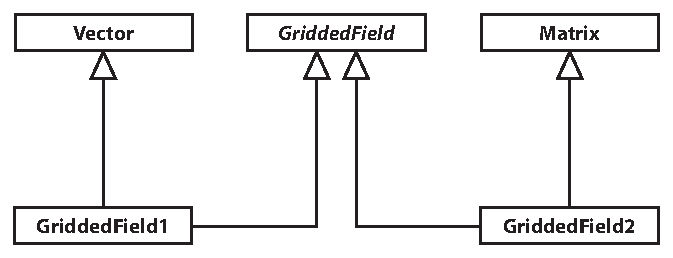
\includegraphics{Figs/development/griddedfields_inheritance}
\caption{UML diagram of gridded field inheritance.}
\label{fig:griddedfields:uml}
\end{center}
\end{figure}


\section{Constructing Gridded Fields}
%-------------------------------------------------------------------------
\label{sec:griddedfields:construct}


\subsection{Creation}
%-------------------------------------------------------------------------
\label{sec:griddedfields:create}

Each \shortcode{GriddedFieldX} offers two constructors. One default
constructor that creates an unnamed gridded field and a second constructor
that takes a string with the name of the gridded field as an argument.

\begin{code}
GriddedField1 gfone("I'm a GriddedField1");
GriddedField2 gftwo;

gftwo.set_name ("I'm a GriddedField2");
\end{code}


\subsection{Initializing the grids}
%-------------------------------------------------------------------------
\label{sec:griddedfields:initgrids}

Once a gridded field has been created, we can start setting up the
grids. There are two different types of grids, a numeric grid and a
string grid. In the following example we set up two gridded fields: A
\builtindoc{GriddedField1} with a numeric grid and a \builtindoc{GriddedField2}
with a numeric grid for the rows and a string grid for the columns. Each grid
can be assigned a name to describe its contents or unit.

\begin{code}
Vector gfonegrid(1,5,1);        // gfonegrid = [1,2,3,4,5]
gfone.set_grid(0, gfonegrid);   // Set grid for the vector elements.

Vector gftwogrid0(1,5,1);       // gftwogrid0 = [1,2,3,4,5]
ArrayOfString gftwogrid1{"Chan1", "Chan2", "Chan3"};

gftwo.set_grid(0, gftwogrid0);  // Set grid for the matrix rows.
gftwo.set_grid(1, gftwogrid1);  // Set grid for the matrix columns.

gfone.set_grid_name (0, "Pressure");

gftwo.set_grid_name (0, "Pressure");
gftwo.set_grid_name (1, "Channel");
\end{code}

\subsection{Initializing the data}
%-------------------------------------------------------------------------
\label{sec:griddedfields:initdata}

The data of a \shortcode{GriddedFieldX} can be accessed through its \shortcode{data} member.
For a \builtindoc{GriddedField1} \shortcode{data} is a \builtindoc{Vector}, for a \builtindoc{GriddedField2} a \builtindoc{Matrix}, for a \builtindoc{GriddedField3} a \builtindoc{Tensor3}, and so on.

The following code shows how to fill the gridded fields from the previous example with data:

\begin{code}
Vector avector(1,4,0.5);    // avector = [1,1.5,2,2.5]

gfone.data = avector;

Matrix amatrix(5,3,4.);     // amatrix = [[4,4,4],[4,4,4],...]

gftwo.data = amatrix;
\end{code}

\subsection{Consistency check}
%-------------------------------------------------------------------------
\label{sec:griddedfields:consistency}

After initializing or changing either the grids or the data, it can happen
that the size of the grids does not match the size of the data anymore. Each
gridded field provides a convenience function which can be called to perform a
consistency check.

\begin{code}
if (!gfone.checksize())
  cout << gfone.get_name()
       << ": Sizes of grid and data don't match" << endl;

// This should fail!
if (!gftwo.checksize())
  cout << gftwo.get_name()
       << ": Sizes of grids and data don't match" << endl;
\end{code}

The complete source code of the examples from this chapter can be found in
\shortcode{src/test\_gridded\_fields.cc}.

%%% Local Variables:
%%% mode: latex
%%% TeX-master: "arts_developer"
%%% End:


\graphicspath{{Figs/interpolation/}}
%
% To start the document, use
%  \chapter{...}
% For lover level, sections use
%  \section{...}
%  \subsection{...}
%
\chapter{\textindex{Interpolation}}
%-------------------------------------------------------------------------
\label{sec:interpolation}


%
% Document history, format:
%  \starthistory
%    date1 & text .... \\
%    date2 & text .... \\
%    ....
%  \stophistory
%
\starthistory
  100204 & Added documentation of grid checking functions by Stefan Buehler.\\
  020528 & Created by Stefan Buehler.\\
\stophistory




%
% Introduction
%

There are no general single-step interpolation functions in ARTS.
Instead, there is a set of useful utility functions that can be used
to achieve interpolation. Roughly, you can separate these into
functions determining grid position arrays, functions determining
interpolation weight tensors, and functions applying the
interpolation. Doing an interpolation thus requires a chain of
function calls:
\begin{enumerate}
\item \funcindex{gridpos} (one for each interpolation dimension)
\item \funcindex{interpweights}
\item \funcindex{interp}
\end{enumerate}
Currently implemented in ARTS is multilinear interpolation in up to 6
dimensions. (Is the 6D case called hexa-linear interpolation?)  The
necessary functions and their interaction will be explained in this
chapter.

\section{Implementation files}
%-------------------------------------------------------------------------

Variables and functions related to interpolation are defined in the files:
\begin{itemize}
\item \fileindex{interpolation.h}
\item \fileindex{interpolation.cc}
\item \fileindex{test\_interpolation.cc}
\end{itemize}
The first two files contain the declarations and implementation, the
last file some usage examples.

\section{Green and blue interpolation}
%-------------------------------------------------------------------------

\begin{figure}[htbp]
  \centering
  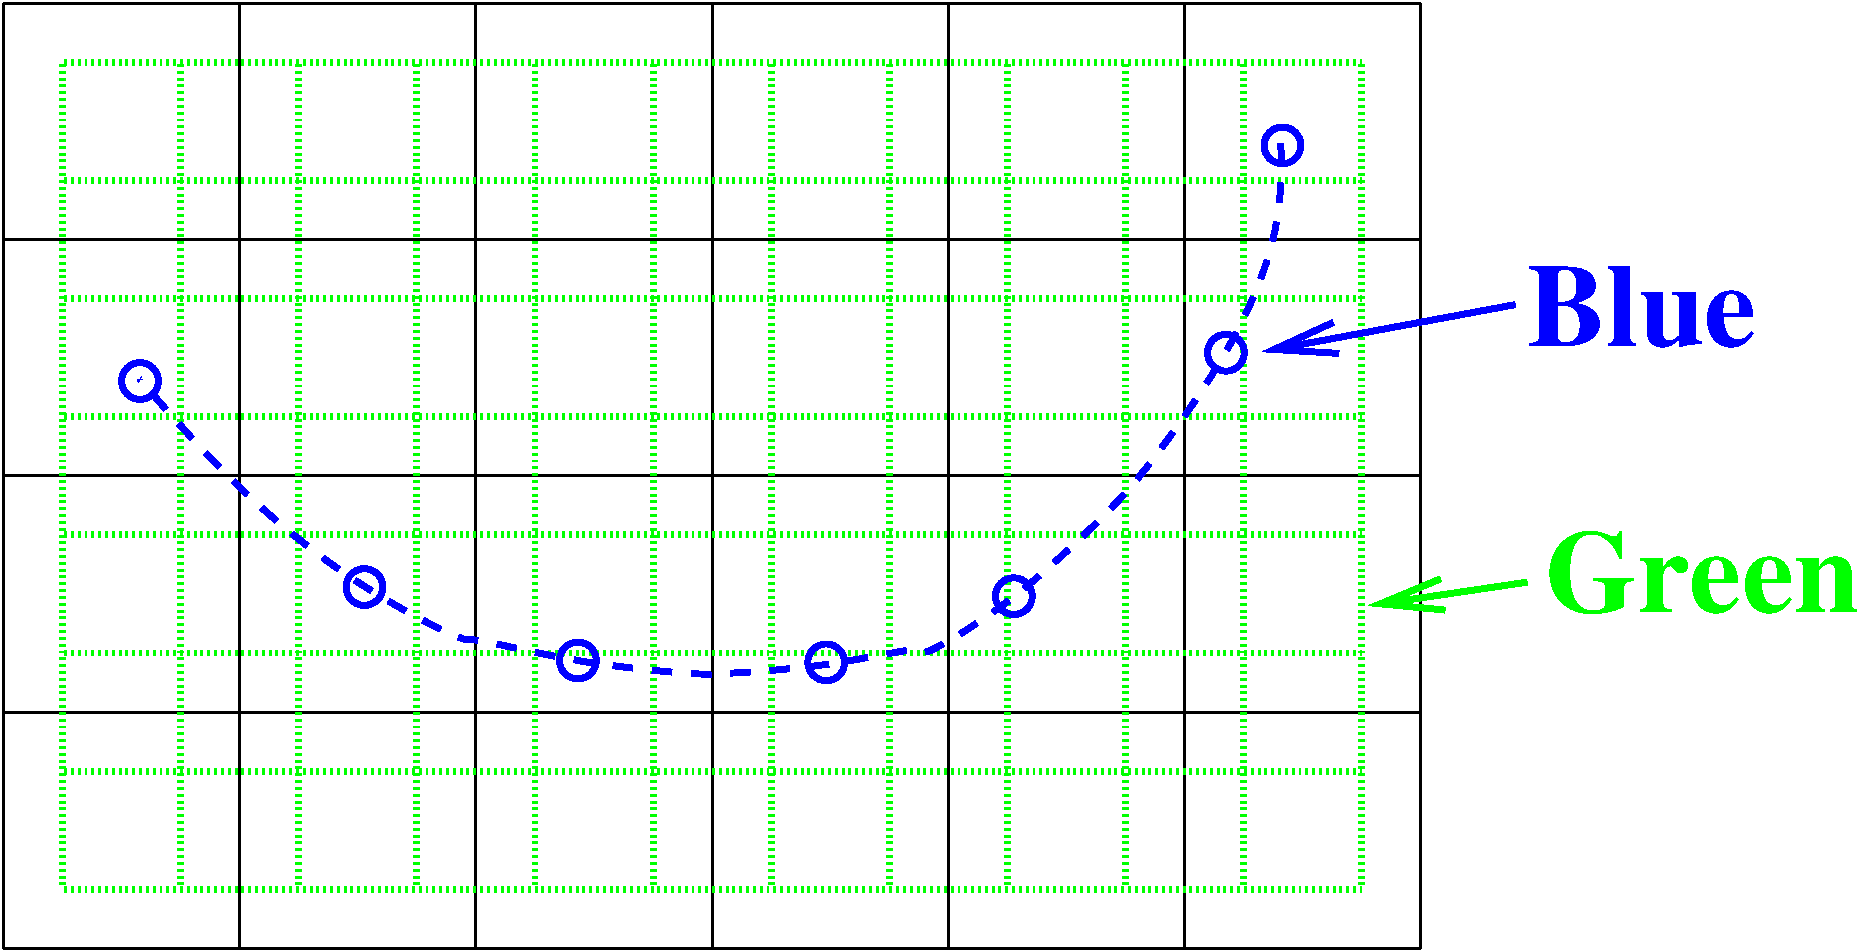
\includegraphics[width=.6\hsize]{interpolation_types}
  \caption{The two different types of interpolation. Green (dotted):
    Interpolation to a new grid, output has same dimension as input,
    in this case 2D. Blue (dashed): Interpolation to a sequence of
    points, output is always 1D.}
  \label{fig:interpolation:types}
\end{figure}

There are two different types of interpolation in ARTS:
\begin{description}
\item[\textindex{Green Interpolation}:] Interpolation of a gridded field to a new
  grid.
\item[\textindex{Blue Interpolation}:] Interpolation of a gridded field to a
  sequence of positions.
\end{description}
Figure \ref{fig:interpolation:types} illustrates the different types
for a 2D example. 

The first step of an interpolation always consists in determining
where your new points are, relative to the original grid. You can do
this separately for each dimension. The positions have to be stored
somehow, which is described in the next section.

\section{Grid checking functions}
%-------------------------------------------------------------------------
\label{sec:interpolation:gridchecking}

Before you do an interpolation, you should check that the new grid is
inside the old grid. (Or only slightly outside.) You can use the
convenience function \funcindex{chk\_interpolation\_grids} for this
purpose, which resides in file \fileindex{check\_input.cc}. The
function has the following parameters:

\begin{code}
const String&     which_interpolation   A string describing the 
                                        interpolation for which 
                                        the grids are intended. 
ConstVectorView   old_grid              The original grid.
ConstVectorView   new_grid              The new grid.
const Numeric&    extpolfac             The extrapolation fraction. 
                                        See gridpos function for 
                                        details. Has a default 
                                        value, which is consistent 
                                        with gridpos.  
\end{code}

There is also a special version for the case that the new grid is just
a scalar. What the function does is check if old and new grid for an
interpolation are ok. If not, it throws a detailed runtime error
message. 

The parameter \shortcode{extpolfac} determines how much extrapolation
is tolerated. Its default value is 0.5, which means that we allow
extrapolation as far out as half the spacing of the last two grid
points on that edge of the grid.

The \shortcode{chk\_interpolation\_grids} function is quite thorough.
It checks not only the grid range, but also the proper sorting,
whether there are duplicate values, etc.. It is not completely cheap
computationally. Its intended use is at the beginning of workspace
methods, when you check the input variables and issue runtime errors
if there are any problems. The runtime error thrown also explains in
quite a lot of detail what is actually wrong with the grids.
  

\section{Grid positions}
%-------------------------------------------------------------------------
\label{sec:interpolation:gridpos}

A grid position specifies where an interpolation point is, relative
to the original grid. It consists of three parts, an \builtindoc{Index} giving the
original grid index below the interpolation point, a \builtindoc{Numeric}
giving the fractional distance to the next original grid point, and a
\builtindoc{Numeric} giving 1 minus this number. Of course, the last element is
redundant. However, it is efficient to store this, since it is used
many times over. We store the two numerics in a plain C array of
dimension 2. (No need to use a fancy Array or Vector for this, since
the dimension is fixed.) So the structure \typeindex{GridPos} looks like:

\begin{code}
struct GridPos  {
   Index   idx;      /*!< Original grid index below
                          interpolation point. */
   Numeric fd[2];    /*!< Fractional distance to next point
                          (0<=fd[0]<=1), fd[1] = 1-fd[0]. */ 
};
\end{code}

For example, \shortcode{idx}=3 and \shortcode{fd}=0.5 means that this interpolation point is
half-way between index 3 and 4 of the original grid.  Note, that
`below' in the first paragraph means `with a lower index'. If the
original grid is sorted in descending order, the value at the grid
point below the interpolation point will be numerically higher than
the interpolation point.  In other words, grid positions and
fractional distances are defined relative to the order of the original
grid. Examples:

\begin{code}
old grid = 2 3
new grid = 2.25
idx      = 0
fd[0]    = 0.25

old grid = 3 2
new grid = 2.25
idx      = 0
fd[0]    = 0.75
\end{code}

Note that \shortcode{fd[0]} is different in the second case, because the old grid
is sorted in descending order. Note also that \shortcode{idx} is the same in
both cases.

Grid positions for a whole new grid are stored in an \shortcode{Array<GridPos>}
(called \shortcode{ArrayOfGridPos}). 

\section{Setting up grid position arrays}
%----------------------------------------------------------------------

There is only one function to set up grid position arrays, namely 
\funcindex{gridpos}:

\begin{code}
void gridpos( ArrayOfGridPos& gp,
              ConstVectorView old_grid,
              ConstVectorView new_grid 
              const Numeric&  extpolfac=0.5 );
\end{code}

\hspace{-\parindent}Some points to remember:
\begin{itemize}
\item As usual, the output \shortcode{gp} has to have the right dimension. 
  
\item The old grid has to be strictly sorted. It can be in ascending
  or descending order. But there must not be any duplicate values.
  Furthermore, the old grid must contain at least two points.
  
\item   The new grid does not have to be sorted, but the function will be
  faster if it is sorted or mostly sorted. It is ok if the new grid
  contains only one point.
  
\item   The beauty is, that this is all it needs to do also interpolation in
  higher dimensions: You just have to call gridpos for all the
  dimensions that you want to interpolate.
  
\item   Note also, that for this step you do not need the field itself at
  all!

\item   If you want to use the returned gp object for something else
  than interpolation, you should know that gridpos guarantees the
  following:\newline
  For the ascending old grid case: 
   \begin{code}
   old_grid[tgp.idx]<=tng || tgp.idx==0
   \end{code}

  And for the descending old grid case: 
   \begin{code}
   old_grid[tgp.idx]>=tng || tgp.idx==0
   \end{code}

\item   Finally, note that parameter \shortcode{extpolfac} plays the
  same role as explained above in Section
  \ref{sec:interpolation:gridchecking}. 
\end{itemize}

\section{\textindex{Interpolation weights}}
%----------------------------------------------------------------------

As explained in the `Numerical Recipes'
\citep{numerical_recipes_C:97}, 2D bi-linear interpolation means, that
the interpolated value is a weighted average of the original field at
the four corner points of the grid square in which the interpolation
point is located. Taking the corner points in the order indicated in Figure
\ref{fig:interpolation:square}, the interpolated value is given by:
\begin{eqnarray}
  y(t,u)
  &=& (1-t)*(1-u)*y_1 \nonumber \\
  & & \mbox{} + t*(1-u)*y_2 \nonumber \\
  & & \mbox{} + (1-t)*u*y_3 \nonumber \\
  & & \mbox{} + t*u*y_4 \nonumber \\
  &=& w_1*y_1 + w_2*y_2 + w_3*y_3 + w_4*y_4
\label{eq:interpolation:weights}
\end{eqnarray}
where $t$ and $u$ are the fractional distances between the
corner points in the two dimensions, $y_i$ are the field values
at the corner points, and $w_i$ are the interpolation weights.

\begin{figure}
  \centering
  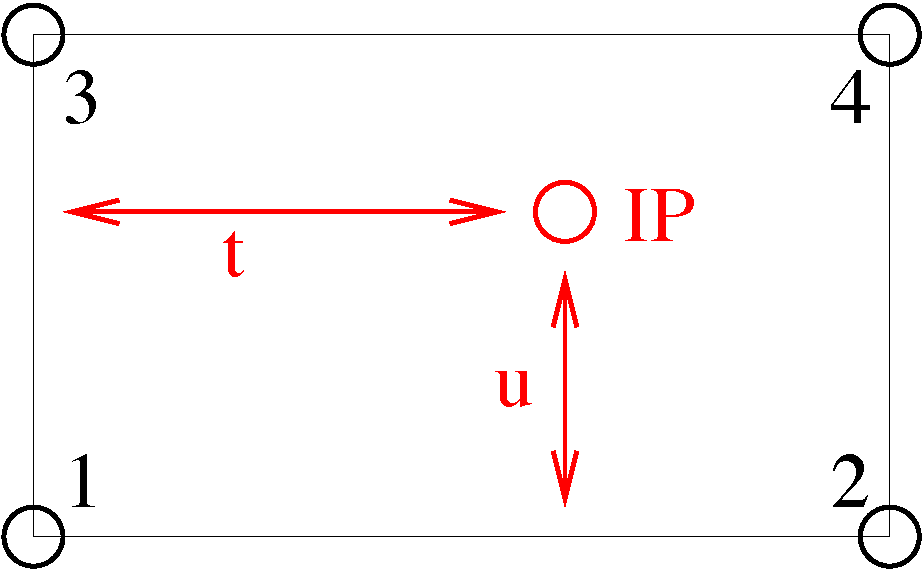
\includegraphics[width=.4\hsize]{interpolation_square}
  \caption{The grid square for 2D interpolation. The numbers 1\ldots 4
    mark the corner points, IP is the interpolation point, $t$ and $u$
    are the fractional distances in the two dimensions.}
  \label{fig:interpolation:square}
\end{figure}

(By the way, I have discovered that this is exactly the result that
you get if you first interpolate linearly in one dimension, then in
the other. I was playing around with this a bit, but it is the more
efficient way to pre-calculate the $w_i$ and do all dimensions at once.

How many interpolation weights one needs for a multilinear
interpolation depends on the dimension of the interpolation: There are
exactly $2^n$ interpolation weights for an $n$ dimensional
interpolation.  These weights have have to be computed for each
interpolation point (each grid point of the new grid, if we do a
`green' type interpolation. Or each point in the sequence, if we do a
`blue' type interpolation).

This means, calculating the interpolation weights is not exactly
cheap, especially if one interpolates simultaneously in many
dimensions. On the other hand, one can save a lot by re-using the
weights.  Therefore, interpolation weights in ARTS are stored in a
tensor which has one more dimension than the output field. The last
dimension is for the weight, so this last dimension has the extent 4
in the 2D case, 8 in the 3D case, and so on (always $2^n$).

In the case of a `blue' type interpolation, the weights are
always stored in a matrix, since the output field is always 1D (a
vector). 

\section{Setting up interpolation weight tensors}
%----------------------------------------------------------------------

Interpolation weight tensors can be computed by a family of functions,
which are all called \funcindex{interpweights}. Which function is actually
used depends on the dimension of the input and output quantities. For
this step we still do not need the actual fields, just the grid
positions.

\subsection{Blue interpolation}

In this case the functions are:

\begin{code}
void interpweights( MatrixView itw,
                    const ArrayOfGridPos& cgp );
void interpweights( MatrixView itw,
                    const ArrayOfGridPos& rgp,
                    const ArrayOfGridPos& cgp );
void interpweights( MatrixView itw,
                    const ArrayOfGridPos& pgp,
                    const ArrayOfGridPos& rgp,
                    const ArrayOfGridPos& cgp );
void interpweights( MatrixView itw,
                    const ArrayOfGridPos& vgp,
                    const ArrayOfGridPos& sgp,
                    const ArrayOfGridPos& bgp,
                    const ArrayOfGridPos& pgp,
                    const ArrayOfGridPos& rgp,
                    const ArrayOfGridPos& cgp );
\end{code}

In all cases, the dimension of \shortcode{itw} must be consistent with the
given grid position arrays and the dimension of the interpolation
(last dimension $2^n$). Because the grid position arrays are
interpreted as defining a sequence of positions they must all have
the same length.

\subsection{Green interpolation}

In this case the functions are:

\begin{code}
void interpweights( Tensor3View itw,
                    const ArrayOfGridPos& rgp,
                    const ArrayOfGridPos& cgp );
void interpweights( Tensor4View itw,
                    const ArrayOfGridPos& pgp,
                    const ArrayOfGridPos& rgp,
                    const ArrayOfGridPos& cgp );
void interpweights( Tensor5View itw,
                    const ArrayOfGridPos& bgp,
                    const ArrayOfGridPos& pgp,
                    const ArrayOfGridPos& rgp,
                    const ArrayOfGridPos& cgp );
void interpweights( Tensor6View itw,
                    const ArrayOfGridPos& sgp,
                    const ArrayOfGridPos& bgp,
                    const ArrayOfGridPos& pgp,
                    const ArrayOfGridPos& rgp,
                    const ArrayOfGridPos& cgp );
void interpweights( Tensor7View itw,
                    const ArrayOfGridPos& vgp,
                    const ArrayOfGridPos& sgp,
                    const ArrayOfGridPos& bgp,
                    const ArrayOfGridPos& pgp,
                    const ArrayOfGridPos& rgp,
                    const ArrayOfGridPos& cgp );
\end{code}

In this case the grid position arrays are interpreted as defining the
grids for the interpolated field, therefore they can have different
lengths. Of course, \shortcode{itw} must be consistent with the length of
all the grid position arrays, and with the dimension of the
interpolation (last dimension $2^n$).

\section{The actual interpolation}
%----------------------------------------------------------------------

For this final step we need the grid positions, the
interpolation weights, and the actual fields. For each interpolated
value, the weights are applied to the appropriate original field values
and the sum is taken (see Equation
\ref{eq:interpolation:weights}). The \funcindex{interp} family of functions
performs this step.

\subsection{Blue interpolation}

\begin{code}
void interp( VectorView            ia,
             ConstMatrixView       itw,
             ConstVectorView       a,    
             const ArrayOfGridPos& cgp);
void interp( VectorView            ia,
             ConstMatrixView       itw,
             ConstMatrixView       a,    
             const ArrayOfGridPos& rgp,
             const ArrayOfGridPos& cgp);
void interp( VectorView            ia,
             ConstMatrixView       itw,
             ConstTensor3View      a,    
             const ArrayOfGridPos& pgp,
             const ArrayOfGridPos& rgp,
             const ArrayOfGridPos& cgp);
void interp( VectorView            ia,
             ConstMatrixView       itw,
             ConstTensor4View      a,    
             const ArrayOfGridPos& bgp,
             const ArrayOfGridPos& pgp,
             const ArrayOfGridPos& rgp,
             const ArrayOfGridPos& cgp);
void interp( VectorView            ia,
             ConstMatrixView       itw,
             ConstTensor5View      a,    
             const ArrayOfGridPos& sgp,
             const ArrayOfGridPos& bgp,
             const ArrayOfGridPos& pgp,
             const ArrayOfGridPos& rgp,
             const ArrayOfGridPos& cgp);
void interp( VectorView            ia,
             ConstMatrixView       itw,
             ConstTensor6View      a,    
             const ArrayOfGridPos& vgp,
             const ArrayOfGridPos& sgp,
             const ArrayOfGridPos& bgp,
             const ArrayOfGridPos& pgp,
             const ArrayOfGridPos& rgp,
             const ArrayOfGridPos& cgp);
\end{code}

\subsection{Green interpolation}

\begin{code}
void interp( MatrixView            ia,
             ConstTensor3View      itw,
             ConstMatrixView       a,   
             const ArrayOfGridPos& rgp,
             const ArrayOfGridPos& cgp);
void interp( Tensor3View           ia,
             ConstTensor4View      itw,
             ConstTensor3View      a,   
             const ArrayOfGridPos& pgp,
             const ArrayOfGridPos& rgp,
             const ArrayOfGridPos& cgp);
void interp( Tensor4View           ia,
             ConstTensor5View      itw,
             ConstTensor4View      a,   
             const ArrayOfGridPos& bgp,
             const ArrayOfGridPos& pgp,
             const ArrayOfGridPos& rgp,
             const ArrayOfGridPos& cgp);
void interp( Tensor5View           ia,
             ConstTensor6View      itw,
             ConstTensor5View      a,   
             const ArrayOfGridPos& sgp,
             const ArrayOfGridPos& bgp,
             const ArrayOfGridPos& pgp,
             const ArrayOfGridPos& rgp,
             const ArrayOfGridPos& cgp);
void interp( Tensor6View           ia,
             ConstTensor7View      itw,
             ConstTensor6View      a,   
             const ArrayOfGridPos& vgp,
             const ArrayOfGridPos& sgp,
             const ArrayOfGridPos& bgp,
             const ArrayOfGridPos& pgp,
             const ArrayOfGridPos& rgp,
             const ArrayOfGridPos& cgp);
\end{code}

\section{Examples}
%----------------------------------------------------------------------

\subsection{A simple example}

This example is contained in file \fileindex{test\_interpolation.cc}.

\begin{code}
void test05()
{
  cout << "Very simple interpolation case\n";

  Vector og(1,5,+1);            // 1, 2, 3, 4, 5
  Vector ng(2,5,0.25);          // 2.0, 2,25, 2.5, 2.75, 3.0

  cout << "Original grid:\n" << og << "\n";
  cout << "New grid:\n" << ng << "\n";

  // To store the grid positions:
  ArrayOfGridPos gp(ng.nelem());

  gridpos(gp,og,ng);
  cout << "Grid positions:\n" << gp;

  // To store interpolation weights:
  Matrix itw(gp.nelem(),2);
  interpweights(itw,gp);
    
  cout << "Interpolation weights:\n" << itw << "\n";

  // Original field:
  Vector of(og.nelem(),0);
  of[2] = 10;                   // 0, 0, 10, 0, 0

  cout << "Original field:\n" << of << "\n";

  // Interpolated field:
  Vector nf(ng.nelem());

  interp(nf, itw, of, gp);

  cout << "New field:\n" << nf << "\n";
}
\end{code}

\hspace{-\parindent}Ok, maybe you think this is not so simple, but a
large part of the code is either setting up the example grids and
fields, or output. And here is how the output looks like:

\begin{code}
Very simple interpolation case
Original grid:
  1   2   3   4   5
New grid:
  2 2.25 2.5 2.75   3
Grid positions:
   1 0    1
   1 0.25 0.75
   1 0.5  0.5
   1 0.75 0.25
   1 1    0
Interpolation weights:
  1   0
0.75 0.25
0.5 0.5
0.25 0.75
  0   1
Original field:
  0   0  10   0   0
New field:
  0 2.5   5 7.5  10
\end{code}

\subsection{A more elaborate example}

What if you want to interpolate only some dimensions of a tensor,
while retaining others? --- You have to make a loop yourself, but it
is very easy. Below is an explicit example for a more complicated
interpolation case. (Green type interpolation of all pages of a
Tensor3.) This example is also contained in file
\fileindex{test\_interpolation.cc}.

\begin{code}
void test04()
{
  cout << "Green type interpolation of all "
       << "pages of a Tensor3\n";

  // The original Tensor is called a, the new one n. 

  // 10 pages, 20 rows, 30 columns, all grids are: 1,2,3
  Vector  a_pgrid(1,3,1), a_rgrid(1,3,1), a_cgrid(1,3,1); 
  Tensor3 a( a_pgrid.nelem(),
             a_rgrid.nelem(),
             a_cgrid.nelem() ); 
  a = 0;
  // Put some simple numbers in the middle of each page:
  a(0,1,1) = 10;
  a(1,1,1) = 20;
  a(2,1,1) = 30;

  // New row and column grids:
  // 1, 1.5, 2, 2.5, 3
  Vector  n_rgrid(1,5,.5), n_cgrid(1,5,.5); 
  Tensor3 n( a_pgrid.nelem(),
             n_rgrid.nelem(),
             n_cgrid.nelem() ); 

  // So, n has the same number of pages as a, 
  // but more rows and columns.

  // Get the grid position arrays:
  ArrayOfGridPos n_rgp(n_rgrid.nelem()); // For rows.
  ArrayOfGridPos n_cgp(n_cgrid.nelem()); // For columns.

  gridpos( n_rgp, a_rgrid, n_rgrid );
  gridpos( n_cgp, a_cgrid, n_cgrid );

  // Get the interpolation weights:
  Tensor3 itw( n_rgrid.nelem(), n_cgrid.nelem(), 4 );
  interpweights( itw, n_rgp, n_cgp );

  // Do a "green" interpolation for all pages of a:

  for ( Index i=0; i<a.npages(); ++i )
    {
      // Select the current page of both a and n:
      ConstMatrixView ap = a( i,
                              Range(joker), Range(joker) );
      MatrixView      np = n( i,
                              Range(joker), Range(joker) );

      // Do the interpolation:
      interp( np, itw, ap, n_rgp, n_cgp );

      // Note that this is efficient, because interpolation
      // weights and grid positions are re-used.
    }

  cout << "Original field:\n";
  for ( Index i=0; i<a.npages(); ++i )
      cout << "page " << i << ":\n"
           << a(i,Range(joker),Range(joker)) << "\n";

  cout << "Interpolated field:\n";
  for ( Index i=0; i<n.npages(); ++i )
      cout << "page " << i << ":\n"
           << n(i,Range(joker),Range(joker)) << "\n";
}
\end{code}

\hspace{-\parindent}The output is:

\begin{code}
Green type interpolation of all pages of a Tensor3
Original field:
page 0:
  0   0   0
  0  10   0
  0   0   0
page 1:
  0   0   0
  0  20   0
  0   0   0
page 2:
  0   0   0
  0  30   0
  0   0   0
Interpolated field:
page 0:
  0   0   0   0   0
  0 2.5   5 2.5   0
  0   5  10   5   0
  0 2.5   5 2.5   0
  0   0   0   0   0
page 1:
  0   0   0   0   0
  0   5  10   5   0
  0  10  20  10   0
  0   5  10   5   0
  0   0   0   0   0
page 2:
  0   0   0   0   0
  0 7.5  15 7.5   0
  0  15  30  15   0
  0 7.5  15 7.5   0
  0   0   0   0   0
\end{code}


\section{Higher order interpolation}
%----------------------------------------------------------------------

Everything that was written so far in this chapter referred to linear
interpolation, which uses two neighboring data points in the 1D
case. But ARTS also has a framework for higher order polynomial
interpolation. It is defined in the two files

\begin{itemize}
\item \fileindex{interpolation\_poly.h}
\item \fileindex{interpolation\_poly.cc}
\end{itemize}

We define interpolation order $O$ as the order of the polynomial that
is used. Linear interpolation, the ARTS standard case, corresponds to
$O=1$. $O=2$ is quadratic interpolation, $O=3$ cubic interpolation.
The number of interpolation points (and weights) for a 1D
interpolation is $O+1$ for each point in the new grid. So, linear
interpolation uses 2 points, quadratic 3, and cubic 4. 

As a special case, interpolation order $O=0$ is also implemented,
which means `nearest neighbor interpolation'. In other words, the
value at the closest neighboring point is chosen, so there is no real
interpolation at all. This case is particularly useful if you have a
field that may be interpolated in several dimensions, but you do not
really want to do all dimensions all the time. With $O=0$
interpolation and a grid that matches the original grid, interpolation
can be effectively `turned off' for that dimension.

Note, that if you use even interpolation orders, you will have an
unequal number of interpolation points `to the left' and `to the
right' of your new point. This is an argument for preferring $O=3$ as the
basic higher order polynomial interpolation, instead of $O=2$.

Overall, higher order interpolation works rather similarly to the
linear case.  The main difference is that grid positions for higher
order interpolation are stored in an object of type
\shortcode{GridPosPoly}, instead of \shortcode{GridPos}. A
\shortcode{GridPosPoly} object contains grid indices and interpolation
weights for all interpolation points. For each point in the new grid,
there are $O+1$ indices and $O+1$ weights.

The reason
why we store all interpolation point indices, and not only the index
of the first point, is to allow correct handling of circular
interpolation, for example in scattering phase function $\phi$
angle. If the angle goes from 0 to 360$^\circ$, then points just below
360 should be used in interpolations to points just above 0, so the
indices to use are not contiguous in memory. Functions to handle this
are not yet implemented, but this should be a relatively simple matter.

In contrast to \shortcode{GridPos}, \shortcode{GridPosPoly} stores
weights \shortcode{w} rather than fractional distances \shortcode{fd}.
For the linear case:
\begin{code}
  w[0] = fd[1]
  w[1] = fd[0]
\end{code}

So the two concepts are almost the same.  Because the w are associated
with each interpolation point, they work also for higher interpolation
order, whereas the concept of fractional distance does not.

The weights are calculated according to 
section 3.1, eq. 3.1.1 of \citep{numerical_recipes_C:97}. These are
for the 1D case. For 2D and higher dimensional cases, the weights of
the individual dimensions have to be multiplied, just as in the linear
interpolation case.

Instead of \shortcode{gridpos}, you have to use the function
\shortcode{gridpos\_poly} for higher order interpolation. It works
exactly like \shortcode{gridpos}, but has an additional argument that
gives the interpolation order $O$. 

After setting up the \shortcode{GridPosPoly} object with
\shortcode{gridpos\_poly}, you have to call \shortcode{interpweights}
and \shortcode{interp}, exactly as in the linear case. (The actual
functions used are not the same, since the name is overloaded. The
\shortcode{interpweights} and \shortcode{interp} functions for use
with \shortcode{GridPosPoly} are implemented in
\shortcode{interpolation\_poly.cc}.) So, a complete interpolation chain
involves:

\begin{code}
gridpos_poly
interpweights
interp
\end{code}

For $O=1$ the result of the
interpolation chain will be the same as for the linear interpolation
routines. Below is a simple complete example, taken from
the file \fileindex{test\_interpolation.cc} in the arts source directory: 

\begin{code}
void test08()
{
  cout << "Very simple interpolation case for the "
       << "new higher order polynomials.\n";

  Vector og(1,5,+1);            // 1, 2, 3, 4, 5
  Vector ng(2,5,0.25);          // 2.0, 2,25, 2.5, 2.75, 3.0

  cout << "Original grid:\n" << og << "\n";
  cout << "New grid:\n" << ng << "\n";

  // To store the grid positions:
  ArrayOfGridPosPoly gp(ng.nelem());

  Index order=2;                // Interpolation order.

  gridpos_poly(gp,og,ng,order);
  cout << "Grid positions:\n" << gp;

  // To store interpolation weights:
  Matrix itw(gp.nelem(),order+1);
  interpweights(itw,gp);
    
  cout << "Interpolation weights:\n" << itw << "\n";

  // Original field:
  Vector of(og.nelem(),0);
  of[2] = 10;                   // 0, 0, 10, 0, 0

  cout << "Original field:\n" << of << "\n";

  // Interpolated field:
  Vector nf(ng.nelem());

  interp(nf, itw, of, gp);

  cout << "New field (order=" << order << "):\n" << nf << "\n";  

  cout << "All orders systematically:\n";
  for (order=1; order<5; ++order)
    {
      gridpos_poly(gp,og,ng,order);
      itw.resize(gp.nelem(),order+1);
      interpweights(itw,gp);
      interp(nf, itw, of, gp);

      cout << "order " << order << ": ";
      for (Index i=0; i<nf.nelem(); ++i)
        cout << setw(8) << nf[i] << " ";
      cout << "\n";
    }
}
\end{code}



\section{Summary}
%----------------------------------------------------------------------

Now you probably understand better what was written at the very
beginning of this chapter, namely that doing an interpolation always
requires the chain of function calls:
\begin{enumerate}
\item \shortcode{gridpos} or \shortcode{gridpos\_poly} (one for each interpolation dimension)
\item \shortcode{interpweights}
\item \shortcode{interp}
\end{enumerate}
If you are interested in how the functions really work, look in file
\fileindex{interpolation.cc} or \fileindex{interpolation\_poly.cc}.
The documentation there is quite detailed.  When you are using
interpolation, you should always give some thought to whether you can
re-use grid positions or even interpolation weights. This can really
save you a lot of computation time. For example, if you want to
interpolate several fields --- which are all on the same grids --- to
some position, you only have to compute the weights once.


%%% Local Variables: 
%%% mode: latex 
%%% TeX-master: "arts_developer" 
%%% End:


\chapter{Integration functions}
%--------------------------------------------------------------------------
\label{sec:integration}

\starthistory
  220802 & Created and written by Sreerekha T.R.\\
  220103 & Included mathematical description for implemented integration method(CE).\\
\stophistory

%
% Introduction
%
A radiative transfer model which takes into account the effect of
scattering involves integration of certain quantities over the angles
of observation.  For example, from Section
\ref{sec:doit:VRTE_sol} it is clear that computing
scattering cross-section and scattering integral term requires
integration over zenith and azimuth directions. There are a wide range
of methods that can be used for numerical integration. They can be
used depending on various factors starting from how accurate the
result should be to the behaviour of the function. The one which is
implemented in ARTS is the trapezoidal integration method.


\section{Implementation files}
%-------------------------------------------------------------------------
\label{sec:integration:files}

The integration functions can be found in the files:
\begin{itemize}
\item \fileindex{math\_funcs.h}
\item \fileindex{math\_funcs.cc}
\end{itemize}
The implementation function \shortcode {AngIntegrate\_trapezoid}is
discussed in the second file. 

\section{Trapezoidal Integration}
%------------------------------------------------------------------------
\label{sec:integration:trapezoidal}

Trapezoidal Integration method comes under the Newton-Cotes formulas
where integration of a function is approximated by the area under the
curve described by the function.  Trapezoidal integration assumes that
the area under the curve is trapezoid.  

Trapezoidal rule : 
\begin{eqnarray}
\label{eq:trapezoidal_rule}
{\int_{x_1}^{x_2} f(x)dx}  = \frac{1}{2} h (f_1 + f_2) + O(h^3 f^{''})
\end{eqnarray}
This is a two-point formula ($x_1$ and $x_2$).  It is exact for
polynomials upto and including degree 1, i.e., f(x) = x. $O(h^3
f^{''})$ signifies how far is the true answer from the estimate. 

If we use eq. \ref{eq:trapezoidal_rule} $N - 1$ times, to do the
integration in the intervals $(x_1, x_2)$,  $(x_2, x_3)$, ...,
$(x_{N-1}, x_N)$, and then add the results, we obtain extended formula
for the integral from $x_1$ to $x_N$.

Extended Trapezoidal rule :
\begin{eqnarray}
\label{eq:ext_trapezoidal_rule}
{\int_{x_1}^{x_N} f(x)dx}  = \frac{1}{2} h \left [f_1 + 2(f_2 + f_3 +
... +f_{N-1})+f_N \right] + O\left [ \frac {(b-a)^3 f^{''}}{N^2} \right]
\end{eqnarray}

The last term tells how much the error will be decreased by taking
more number of steps. 

\section{Solid Angle Integration}
%------------------------------------------------------------------------
\label{sec:integration:solid_angle}
In our scattering problem, we are often encountered with a double integration
of functions over zenith and azimuth angles (see Chapter
\ref{sec:doit}).  One way to achieve
double integration is to use repeated
one-dimensional trapezoidal integration.  This is effective of course
only if the boundary is simple and the function is very smooth.  If
the function is strongly peaked and if know where it occurs, integral
should be broken into smaller regions so that the 
integrand is smooth in each.  Another thing is to take into account
the symmetry of the function as well as the boundary. For example in
our case, if the radiation is symmetric about the azimuth, the
integration in that direction returns constant value of $2 \pi$ and we
need to do only integration over zenith directions.  

The general form of a solid angle integration is
\begin{equation}
  \label{eq:solid_int}
S = \int_{4\pi} f(\omega) \DiffD\omega
\end{equation}
In spherical coordinates we can write:
\begin{equation}
  \label{eq:sol_int_sph}
 S = \int_0^\pi \int_0^{2\pi} f(\theta,\phi) \sin\theta \quad\DiffD\theta\DiffD\phi
\end{equation}
A double integration can be splitted into two single integrations:
\begin{eqnarray}
 S &=& \int_0^\pi \left(\int_0^{2\pi}  f(\theta,\phi) \sin\theta \DiffD\phi \right) \DiffD\theta \\
 &=& \int_0^\pi g(\theta) \DiffD\theta
\end{eqnarray}
If we have to integrate a vector, we can apply this method componentwise.

To solve the integral numerically we discretize $\theta$ and $\phi$ and obtain two angular grids ( $[\theta_0, \theta_1, \cdots, \theta_n]$  and $[\phi_0, \phi_1, \cdots, \phi_m]$). 
Then we can first calculate $g(\theta_j)$ for all $\theta_j$ unsing the trapezoidal method.
\begin{equation}
  g(\theta_j) = \sum_{i=1}^m \sin\theta_j \frac{f(\theta_j, \phi_i) + f(\theta_j, \phi_{i+1})}{2} \cdot (\phi_{i+1} - \phi_i)  
\end{equation}
The final step is to sum up all $g(\theta_j)$, again applying the trapezoidal method.
\begin{equation}
  S = \sum_{j=1}^n \frac{g(\theta_j) + g(\theta_{j+1})}{2} \cdot  (\theta_{j+1} - \theta_j)  
\end{equation}

If the radiation is symmetric about the azimuth we just calculate:
\begin{equation}
  S_{sym} = 2\pi \int_0^{\pi} f(\theta) \sin(\theta) \DiffD \theta 
\end{equation}
Unsing the trapezoidal method this can be written as:
\begin{equation}
  S_{sym} =  2\pi \sum_{j=1}^n \frac{h(\theta_j) + h(\theta_{j+1})}{2} \cdot  (\theta_{j+1} - \theta_j)  
\end{equation}
where $h(\theta) = \sin\theta\cdot f(\theta)$.
 
\vspace{2ex}



The function  \shortcode{AngIntegrate\_trapezoid} takes as input the integrand and the angles over which
the integration has to be done. For example in this case it can be the
zenith and azimuth angle
grid.
\begin{code}  
Numeric AngIntegrate_trapezoid(MatrixView Integrand,
                               ConstVectorView za_grid,
                               ConstVectorView aa_grid)
\end{code}
The integrand has the same number of rows as zenith angle grid
and columns as azimuth angle grid.  The inner loop does trapezoidal
integration of the integrand over all azimuth angles and the result is
stored in a Vector  res1[i]. Note that the integrand at every point
has to be multiplied with \shortcode {sin (za\_grid[i] * DEG2RAD)}
since we are integrating over solid angles.  The outer loop 
does an integration of res1[i] over all zentih angles.  The result of
this is returned back to the calling function.  


%%% Local Variables: 
%%% mode: latex
%%% TeX-master: t
%%% End: 

\chapter{Linear algebra functions}
%--------------------------------------------------------------------------
\label{sec:lin_alg}

\starthistory
  020502 & Created and written by Claudia Emde.\\
\stophistory

%
% Introduction
%

Solving the vector radiative transfer equation requires the
computation of linear equation systems and the matrix
exponential. This section describes the functions which are implemented
in ARTS and it gives instructions how these functions can be used, also
for other purposes than the radiative transfer calculations.

\section{Implementation files}
%-------------------------------------------------------------------------
\label{sec:lin_alg:files}

All the functions described below can be found in the files:
\begin{itemize}
\item \fileindex{lin\_alg.h}
\item \fileindex{lin\_alg.cc}
\end{itemize}
The template class \shortcode{Array} and the classes \builtindoc{Matrix} and
\builtindoc{Vector} are used, therefore the linear algebra functions require
the files:
\begin{itemize}
\item \fileindex{matpackI.h}
\item \fileindex{make\_vector.h}
\item \fileindex{array.h}
\item \fileindex{matpackI.cc}
\item \fileindex{make\_vector.cc}
\item \fileindex{array.cc}
\end{itemize}
Furthermore logical functions contained in
\begin{itemize}
\item \fileindex{logic.h}
\item \fileindex{logic.cc}
\end{itemize}
are used to check the dimensions of input matrices for various functions.


\section{Linear Equation Systems}
%------------------------------------------------------------------------
\label{sec:lin_alg:lineqsys}


For solving a set of linear equations 
\begin{eqnarray}
\label{eq:lin_equ_sys}
{\bf A} {\bf x} = {\bf b}
\end{eqnarray}
the LU decomposition method is implemented.A slightly modified version
of the algorithm described in
[\cite{numerical_recipes_C:97}] is used here. An alternative method
is the Gauss-Jordan elimination, but this method is three times
slower than the LU decomposition method
[\cite{numerical_recipes_C:97}, p.36]. The LU decomposition method
reqires two functions, \shortcode{ludcmp} and \shortcode{lubacksub},
which will be decribed below.
\vspace{0.5cm}\\
The following example for a three dimensional equation sytem 
demonstrates how to solve a linear
equation sytem of the type
(\ref{eq:lin_equ_sys}):
\begin{itemize}
\item Create matrix A, vector b: \\
  \shortcode{A = Matrix(3,3);} \\
  \shortcode{A(1,1) = 4;}\\
  \shortcode{A(2,1) = 3;}\\
  $\cdots$\\
  \shortcode{b = Vector(3);}\\
  \shortcode{b(1) = 7;}\\
  $\cdots$
\item Initialize solution vector x and two other variables needed for
  storing intermediate results:\\
  \shortcode{x = Vector(3);}\\
  \shortcode{LU = Matrix(3,3);}\\
  \shortcode{indx = ArrayOfIndex(3);}
\item Call LU decomposition function (see Section \ref{sec:lin_alg:lu_decomp}): \\
  \shortcode{ludcmp(LU, indx, A);}
\item Call LU backsubstitution function (see Section \ref{sec:lin_alg:backsub}): \\
  \shortcode{lubacksub(x, LU, b, indx);}
\item Print the solution vector:\\
  \shortcode{cout << x;}
\end{itemize}

\subsection{LU Decomposition}
%------------------------------------------------------------------------
\label{sec:lin_alg:lu_decomp}

A LU decomposition is a procedure for decomposing a square matrix {\bf
  A} with
dimension $n$ into a product of a lower triangular matrix {\bf L} (has
elements only on the diagonal elements and below) and
an upper triangular matrix {\bf U} (has elements only on the diagonal
and above):
\begin{equation}
  \label{eq:lu_decomp}
  {\bf L}\cdot{\bf U} ={\bf A} 
\end{equation}
For a 3 x 3 matrix equation \ref{eq:lu_decomp} would look like this: 
\[ \left(
  \begin{array}{ccc}
    l_{11} & 0 & 0 \\
    l_{21} & l_{22} & 0 \\
    l_{31} & l_{32} & l_{33}
    \end{array} \right)
\cdot
\left(
  \begin{array}{ccc}
    u{11} & u_{12} & u_{13} \\
    0 & u_{22} & u_{23}\\
    0 & 0 & u_{33}
    \end{array} \right)
=
\left(
  \begin{array}{ccc}
    a_{11} & a_{12} & a_{13} \\
    a_{21} & a_{22} & a_{23} \\
    a_{31} & a_{32} & a_{33}
    \end{array} \right)
\]
The decomposition can be used to rewrite the linear set of equations
(\ref{eq:lin_equ_sys}) in the following way:
\begin{eqnarray}
  {\bf A}\cdot{\bf x} = ({\bf L}\cdot{\bf U})\cdot{\bf x} = {\bf
    L}\cdot({\bf U}\cdot{\bf x}) = {\bf b}
\end{eqnarray}
First 
\begin{equation}
  {\bf L} \cdot{\bf y} = {\bf b}
\end{equation}
is solved for the vector ${\bf y}$ which can be done by
forward substitution (see section \ref{sec:lin_alg:backsub}). Then 
\begin{equation}
  {\bf U} \cdot{\bf x} = {\bf y}
\end{equation}
is solved again by backsubstitution. 
The advantage in breaking up one linear set into two successive ones
is that the solution of a triangular set of equations is quite trivial.

The function \shortcode{ludcmp} requires a square matrix of arbitrary
dimension $n$ as input and performs the LU decomposition. It returns one
matrix which contains both matrices, ${\bf L}$ and ${\bf U}$. 
For the lower triangular matrix  ${\bf L}$ the diagonal elements 
are chosen to be 1, then the other elements of ${\bf L}$ and ${\bf U}$
are determined. This is possible, as the LU decomposition is an under
determined equation sytem with $n^2$ equations for $n^2+n$ unknowns. 
The output matrix does not include the diagonal of ${\bf L}$, in the
three-dimensional case it has the following elements:
\[ \left(
  \begin{array}{ccc}
    u_{11} & u_{12} & u_{13} \\
    l_{21} & u_{22} & u_{23} \\
    l_{31} & l_{32} & u_{33}
    \end{array} \right)
\]
This special arrangement of the LU decomposition is named {\sl
Crout's algorithm} and a matrix arranged in this form is named {\sl
Crout matrix} in this context.
  

Another output variable of the function \shortcode{ludcmp} is an index
vector which contains information about pivoting which is absolutely
essential for the stability of
Crout's algorithm. Here partial pivoting,
i.e. interchange of rows is implemented. That means that not {\bf A} is
decomposed into $LU$-form but a rowwise permutation of {\bf A}. If the
index vector contains for example the elements $(2,1,0)$ the first and
the last row of a three dimensional matrix would be exchanged.


\subsection{Forward- and Backsubstitution}
%---------------------------------------------------------------
\label{sec:lin_alg:backsub}
An equation system of the form
\[ 
\left(
  \begin{array}{ccc}
    a{11} & a_{12} & a_{13} \\
    0 & a_{22} & a_{23}\\
    0 & 0 & a_{33}
    \end{array} \right)
\cdot
\left(
  \begin{array}{c}
    x_1\\x_2\\x_3
 \end{array} \right)
=
\left(
  \begin{array}{c}
    b_1\\b_2\\b_3
 \end{array} \right)
\]
can be solved very easy. The last element, here $x_3$, is already isolated,
namely
\begin{eqnarray}
  x_3 = b_3/a_{33}
\end{eqnarray}
As $x_3$ is known $x_2$ can be calculated using the second row of the
eqautions. Then, finally, $x_1$ can be calculated as well using the
first row. This procedure
is called backsubtitution. The same
method  applied for an equation system including a
lower triangular matrix is named forward substitution.   

The function \shortcode{lubacksub} does forward and backward
substitution to solve the equation system described in
\ref{sec:lin_alg:lu_decomp}. As input it requires the output variables of
\shortcode{ludcmp} which are the {\sl Crout matrix} and the index
vector. Output of the function is the solution vector ${\bf x}$ to the
equation system.


\subsection{More Applications of the LU Decomposition}
%-------------------------------------------------------------------
\label{lu_applications}

\begin{itemize}
\item Inverse of a matrix:\\
  To compute $(\bf K)^{-1}\cdot{\bf b}$, which is a part of the
solution to the vector radiative transfer equation (Equation
\ref{U-eq:scattering:VRTE_sol} in \user) the LU
decomposition method can be used. The following equations show, that
the problem is equivalent to  solving a linear equation system of the type
\ref{eq:lin_equ_sys}.
\begin{eqnarray}
  {\bf K}^{-1}\cdot{\bf b} &=& {\bf x}\\
\Leftrightarrow \qquad  {\bf K}\cdot{\bf x} &=& {\bf b}
\end{eqnarray}

\item To solve the equation system
  \begin{eqnarray}
    {\bf A}\cdot{\bf X} &=& {\bf B}
  \end{eqnarray}
where {\bf A}, {\bf B} and  {\bf X} are matrices of dimension
$n$, the LU decomposition functions can be applied as well. Assume
that {\bf A} and {\bf B} are known and you want to solve for {\bf
 X}.
First you should do a LU decomposition of  {\bf A} and then
backsubstitute with the columns of B and you get the columns of {\bf
  X} as solution vectors.

\end{itemize}

\section{Matrix Exponential Function}
%----------------------------------------------------------------
\label{sec:lin_alg:mat_exp}

A very important function for solving differential equations is the
matrix exponential:
\begin{eqnarray}
  \label{eq:mat_exp}
  e^{{\bf A}s} = \sum_{k=0}^\infty{\frac{({\bf A} s)^k}{k!}}
\end{eqnarray}
In principle it could be computed using the Taylor power series but 
 this method is not efficient. {\sc Moler} and {\sc Van
  Loan} have shown for the simple example [\cite{Moler_Loan:79}]
\[ {\bf A} =
\left(
  \begin{array}{cc}
    -49 & 24\\
    -64 & 31
    \end{array} \right) \]
that convergence is obtained not until 59 terms. And if a relative
accuracy of only 10$^{-5}$ is taken, the method even leads to a wrong
result due to rounding errors.

\subsection{Pad\'e Approximation}
%----------------------------------------------------------------------
\label{sec:pade_approximation}

One of the better algorithms for computing the matrix exponential is
the Pad\'e approximation which is also shortly described in
[\cite{Moler_Loan:79}] and outlined in the book ``Matrix
Computations'' by \cite{Golub_Loan:91}. 
The method uses perturbation theorie as well as the so called Pad\'e
functions. It is possible to derive an algorithm which calculates
\begin{eqnarray}
  {\bf F} = e^{{\bf A}+{\bf E}} 
\end{eqnarray}
where 
\begin{eqnarray}
  \|{\bf E}\|_\infty \le \delta \|{\bf A}\| .
\end{eqnarray}
The accuracy of the computation given by $\delta$ can be chosen. 
The parameter q has to be the smallest non-negative integer such that
$\epsilon(q,q)\le\delta$ where
\begin{eqnarray}
  \epsilon(p,q) = 2^{3-(p+q)}\frac{p!q!}{(p+q)!(p+q+1)!}.
\end{eqnarray}
The following table shows values of epsilon for
different values of q.
\vspace{0.5cm}\\
\begin{tabular}[h]{|r|r|}
 \hline
q & $\epsilon$(q,q) \\ \hline
1 & 0.1667\\
2 & 6.9444 $\cdot$ 10$^{-4}$ \\
3 & 1.2401 $\cdot$ 10$^{-6}$ \\
4 & 1.2302 $\cdot$ 10$^{-9}$ \\
5 & 7.7667 $\cdot$ 10$^{-13}$ \\
6 & 3.3945 $\cdot$ 10$^{-16}$ \\ 
\hline
\end{tabular}
\vspace{0.5cm}\\
The algorithm is implemented in the function \shortcode{matrix\_exp}. Input
to this function is the matrix ${\bf A}$ and the parameter $q$. As output
it gives the matrix ${\bf F}$ which is defined above.\\
The following example shows how to use the \shortcode{matrix\_exp} function:
\begin{itemize}
\item Initialize {\bf A} and assign values:\\
  \shortcode{Matrix A(3,3);}\\
  \shortcode{A(1,1) = 45;}\\
  \shortcode{A(1,2) = 3;}\\
$\cdots$ 
\item Initialize {\bf F}:\\
  \shortcode{Matrix F(3,3);}
\item Give a paramater for the accuracy:\\
  \shortcode{Index q=6;}
\item Call the matrix exponential function:\\
  \shortcode{matrix\_exp(F,A,q);}
\item Print the result: \\
  \shortcode{cout << "exp(A) = " << F;}
\end{itemize}






%%% Local Variables: 
%%% mode: latex
%%% TeX-master: t
%%% End: 

\chapter{Include ARTS in third-party C++}
%--------------------------------------------------------------------------
\label{sec:cpp_api}

\starthistory
  2020-10-06 & Created and written by Richard Larsson.\\
\stophistory

%
% Introduction
%

It is possible to include ARTS in another C++ program using
the \verb|public_arts_interface| and linking to \verb|autoarts.h|.
This will pull in the ARTS public API defined in \verb|agendas.cc|,
\verb|groups.cc|, \verb|methods.cc|, \verb|workspace.cc| as well
as an automatically generated ARTS namespace to your project.

\FIXME{a private Module that imports only the ARTS namespace
       should be added as soon as soon as C++20 becomes norm}

\section{Linking the public interface}
%--------------------------------------------------------------------------
\label{sec:cpp_api:public_linking}

To link the public interface, you need to \verb|add_subdirectory(arts)|
anywhere in your CMake project, where the \verb|arts| directory should contain
a current version of ARTS.

An example (in your projects \verb|CMakeLists.txt|):
\begin{verbatim}
######################################################
# ARTS Custom Executable
add_executable(arts_interface interface.cpp)
target_link_libraries(arts_interface PUBLIC
                      public_arts_interface)
######################################################
\end{verbatim}

At this point, your \verb|interface.cpp| must have
\verb|#include <autoarts.h>| as one of its headers
and you are good to go.

\section{Using the C++ namespace interface}
%--------------------------------------------------------------------------
\label{sec:cpp_api:usage}

The ARTS namespace contains all the interfaces you will need to perform
all operations supported by ARTS.  The namespace defines only a single
top level function call, the  \verb|init(...)| function and a single
top-level type, the ARTS Workspace.  The function is used to generate the ARTS Workspace
upon which all your function calls are made.  The ARTS namespace has several 
sub-namespaces for various purposes.  These are in short:
\begin{itemize}
 \item[Group] Defines the ARTS public type-system.
 \item[Internal] Defines the ARTS internal type-system.
 \item[Var] Defines the ARTS interface type-system,
                  create variables for the ARTS interface, and
                  access automatic variables that are defined in the ARTS Workspace
                  from the start.
 \item[Method] Defines the ARTS methods.  The ARTS methods can only be called
                     using their generic inputs and outputs.
 \item[AgendaMethod] Defines the ARTS methods that can be used by agendas.
                           They return an internal type and are best used directly,
                           with no manual modification.
 \item[AgendaDefine] Defines methods to set the different ARTS agendas.
                           The agendas are checked and ready to be used after these
                           methods are called.
 \item[AgendaExecute] Executes an agenda.
\end{itemize}

If you are using the public interface, you need not be concerned with the types in the sub-namespaces Group and Internal.
\FIXME{Otherwise, these define the basic types you need to use ARTS easily.}
These sub-namespaces are used the same as any other C++ type-system.  The other
namespaces are domain specific.

An interface will generally start with a call to the initialize function.
This could look like:
\begin{verbatim}
  auto ws = init();
\end{verbatim}
After this the order and set of commands that are placed is up to the user.
For sake of ease, \verb|ws| will be used below to indicate a defined 
Workspace.  Also, the access to each sub-namespace will be written as if
operating in the ARTS namespace itself.

\subsection{Var}
%--------------------------------------------------------------------------
\label{sec:cpp_api:usage:variable}
The Var namespace, short for Variable namespace, have three purposes
\begin{enumerate}
 \item Type the Method and Agenda interface
 \item Access common Workspace variables
 \item Create new variables on the Workspace
\end{enumerate}
The types that are defined correspond to the types in Group.
The purpose of these types is to pass input to the functions of
Method and AgendaMethod.  The main way to generate
instances of these variables is by their corresponding \verb|*Create|
function or by simply accessing them via their common Workspace
names.  The only constructor that is recommended to use is the
construction from the corresponding Group, as this can simplify
the access to several methods.  The other two constructors risk
accessing out-of-bound memory, or to deference a null-pointer.

It is highly recommended to not discard created variables, as they
will still occupy memory in the Workspace until the end of the program
and they become impossible to access once discarded.

Examples:
\begin{verbatim}
  // Define an index that is not in the workspace
  Var::Index x{Group::Index(1)};
  
  // Access an index that is in the workspace
  Var::Index y = Var::stokes_dim(ws);
  
  // Create a new index on the workspace
  Var::Index z{Var::IndexCreate(ws, Group::Index{1},
                                "new_index_name")};
\end{verbatim}
Note that \verb|x| will not work as an input to AgendaMethod functions
but it will work as an input to Method functions.  It does not append
to the Workspace.  The other two will work both as inputs to
AgendaMethod and to Method functions.

\subsection{Method}
%--------------------------------------------------------------------------
\label{sec:cpp_api:usage:method}
The Method namespace contains all but the Agenda manipulating methods
defined in \verb|methods.cc|.  These can all be called using the generic
input and outputs.  The inputs and outputs are not guaranteed to be the
same as in the ARTS methods however, because C++ requires inputs with 
default values be placed last in the calling order.  Note that all 
standard inputs and outputs taken from the Workspace must be set on the
Workspace itself and cannot be passed as inputs.  This creates a few
idiosyncrasies compared to how ARTS is used in python or in a normal
controlfile.  

Examples:
\begin{verbatim}
  // Call yCalc (no GIN/GOUT)
  Method::yCalc(ws);
  
  // Call Touch on the wind field (Pure GOUT)
  Method::Touch(ws, Var::wind_u_field(ws));
  Method::Touch(ws, Var::wind_v_field(ws));
  Method::Touch(ws, Var::wind_w_field(ws));
  
  // Set p_grid by VectorNLogSpace
  Var::nelem(ws) = 51;
  Method::VectorNLogSpace(ws, Var::p_grid(ws), 1e+05, 1e-4);
  
  // Save x, y, z from the Var example
  Var::output_file_format(ws) = Group::String{"ascii"};
  Method::WriteXML(ws, x);
  Method::WriteXML(ws, y, Group::String{"extra.xml"});
  Method::WriteXML(ws, z);
\end{verbatim}
All methods requires a Workspace (\verb|ws|) to work.
The first case of the examples calls a function with neither generic input nor generic output --- it cannot take anything other than the Workspace.
The second triplet case of the examples calls Touch on all wind-field variables.  They will have been default-initialized after this process.
The third example shows the idiosyncrasies to other methods of using ARTS.  The Workspace variable \verb|nelem| has been used instead of a generic
input index to define \verb|VectorNLogSpace| --- thus \verb|nelem| must be set manually by the user of the interface.
The last examples uses the fact that many of \verb|WriteXML|'s inputs are default defined.  Since the default value of filename is empty and since
the interface then infers it has the variable name input, the first call to \verb|WriteXML| will generate a file called \verb|arts.in.xml|, the second
call will generate a file called \verb|extra.xml|, and the last call will generate a file called \verb|arts.new_index_name.xml|.  The first part of
the name can be changed by calling \verb|init()| with the corresponding arguments.

As a last note.  Several inputs above automatically generates inputs from standard C++ types, such as \verb|VectorNLogSpace|
generating two \verb|Var::Numeric| from two doubles.  This is a convenient way to use the methods but the user should
be aware that these methods will end up deleting variables in the end, so some care has to be taken when the scope of such
automatic variables is long.

\subsection{AgendaMethod, AgendaDefine, and AgendaExecute}
%--------------------------------------------------------------------------
\label{sec:cpp_api:usage:agenda}
The Agenda namespaces deal with setting and defining Workspace Agendas.
It is only possible to set Workspace Agendas that have been defined as part
of the Workspace at compilation time.  The AgendaMethod namespace contains
the same functions as the Method namespace but returns an Internal::MRecord.
The user of this interface is expected to never manually construct an MRecord.
Instead, this type is meant to only be used when Agendas are defined in the
AgendaDefine namespace.  The AgendaDefine namespace defines a variadic 
function per Agenda in the common Workspace and expects a list of MRecord
to set this Agenda's methods.  Finally, AgendaExecute exists to execute a single
Agenda.  Normally, this is not preferred since Agendas should generally just
be used inside methods, but the option still exists.

Examples:
\begin{verbatim}
  // Define the basic iy_main_agenda emission agenda
  AgendaDefine::iy_main_agenda(ws,
    AgendaMethod::ppathCalc(ws),
    AgendaMethod::iyEmissionStandard(ws));
  
  // Define an empty geo positioning agenda
  AgendaDefine::geo_pos_agenda(ws,
    AgendaMethod::Ignore(ws, Var::ppath(ws)),
    AgendaMethod::VectorSet(ws, Var::geo_pos(ws),
      Var::VectorCreate(ws, {}, "Default")));
\end{verbatim}
The first example simply sets its agenda by using two functions that
complete the inputs/outputs expected of the agenda.  The second example
does not need or want to use \verb|Var::ppath(ws)| so it ignores it.  It also
has the need of a default empty \verb|Var::Vector|.  This variable
has to first be created onto the Workspace before it can be used as an 
input.  Had a pure vector been used instead of the create-function,
a runtime error would occur.  The create function is only invoked once,
since the internal workings of the Agenda just need to have defined
the variable.

Lastly, each AgendaMethod function that has a default generic input will
create a static const Workspace variable of this type upon first call to
the method.  This means that calling such a method will incur a memory cost
that lasts until the end of the program.





\part{Bibliography and Appendices}
%
\bibliography{references}


\part{Index}
%
\printindex


%===   End of report   =====================================================
\end{document}


%%% Local Variables: 
%%% mode: latex
%%% TeX-master: t
%%% End: 
